\documentclass[a4paper, 12pt]{book}
\usepackage[utf8]{inputenc}
\usepackage[spanish]{babel} %español
\usepackage{newtxtext}
\usepackage{graphicx}
\usepackage{amsmath}
\usepackage{amsfonts}
\usepackage{amssymb}
\usepackage{graphicx}
\usepackage{float} %Usar [H] en las imagenes y tablas
\usepackage[hidelinks]{hyperref} %Para clikear las pag webs
\usepackage{listings} % color de los bloques de código
\usepackage{minted}
\usemintedstyle{vs}
\usepackage[dvipsnames]{xcolor} %color de las letras
\setcounter{tocdepth}{4} % Incluye las secciones, subsecciones y subsubsecciones en el indice
% DEFINIENDO COLORES DE LOS CODIGOS
% SQL
\definecolor{codegray}{rgb}{0.5,0.5,0.5}
\definecolor{backcolour}{rgb}{0.95,0.95,0.92}
\lstdefinestyle{estilosql}{
backgroundcolor=\color{backcolour},   
keywordstyle=\color{blue},
numberstyle=\tiny\color{codegray},
basicstyle=\ttfamily\footnotesize,
breakatwhitespace=false,         
breaklines=true,                 
captionpos=b,                    
keepspaces=true,                 
numbers=left,                    
numbersep=5pt,                  
showspaces=false,                
showstringspaces=false,
showtabs=false,
breaklines=true % las lineas de codigo se rompen si son muy largas                  
}
% Python es usado con minted
% R es usado con minted

\begin{document}

\author{Gabriel Pinilla}
\title{Resumen comandos para la Ciencia de Datos}

\frontmatter
\maketitle
\tableofcontents %índice
\mainmatter %Número del capítulo sobre el título
% CAPÍTULOS
%
%	CAPITULO SQL
\chapter{SQL en Postgres}
% \textcolor{blue}{}
\lstset{style=estilosql}
%	SECCION
\section{Notas previas...}
\begin{enumerate}
	\item Al finalizar una consulta se debe terminar con ;.
	\item El texto se debe escribir entre comillas simples o dobles, dependiendo del programa a utilizar.
	\item En SQL, el primer caracter de un string inicia con 1 y se escriben entre comillas simples.
	\item Para insertar comentarios se debe usar --
\end{enumerate}
%	SECCION
\section{Comandos básicos}
%	SUBSECCION
\subsection{Estructura básica de una consulta}
La siguiente consulta muestra la estructura básica y el orden que deben seguir los comandos:
\begin{lstlisting}[language=SQL]
SELECT col-sep-por-coma
FROM conj-de-datos.tabla
WHERE condicion
GROUP BY columnas
HAVING condicion
ORDER BY columnas DESC
LIMIT numero;
\end{lstlisting}
Si se requieren todas las columnas de la tabla, se debe agregar un * después del comando \textcolor{blue}{SELECT}.
%	SUBSECCION
\subsection{Where vs Having}
En esta consulta, la cláusula \textcolor{blue}{WHERE} filtra y después el \textcolor{blue}{GROUP BY} agrupa:
\begin{lstlisting}[language=SQL]
SELECT col-sep-por-coma
FROM conj-de-datos.tabla
WHERE condicion
GROUP BY columnas;
\end{lstlisting}
Sin embargo, en la siguiente consulta el \textcolor{blue}{GROUP BY} agrupa y luego el \textcolor{blue}{HAVING} filtra:
\begin{lstlisting}[language=SQL]
SELECT col-sep-por-coma
FROM conj-de-datos.tabla
GROUP BY columnas
HAVING condicion;
\end{lstlisting}
%	SUBSECCION
\subsection{Crear una base de datos}
Para crear una base de datos:
\begin{lstlisting}[language=SQL]
CREATE DATABASE nom-base-de-datos;
\end{lstlisting}
%	SUBSECCION
\subsection{Crear una tabla}
Para crear una tabla:
\begin{lstlisting}[language=SQL]
CREATE TABLE nom-tabla (
    col1 tipo-de-variable,
    col2 tipo-de-variable,
);
\end{lstlisting}
El comando \textcolor{blue}{CREATE TABLE IF NOT EXISTS} crea una tabla si es que dicha tabla no existe en la base de datos.
%	SUBSECCION
\subsection{Insertar datos a una tabla}
Insertar datos a una tabla ya creada:
\begin{lstlisting}[language=SQL]
INSERT INTO tabla (col-sep-por-coma)
VALUES (valores-sep-por-coma);
\end{lstlisting}
%	SUBSECCION
\subsection{Ver todos los datos}
Para ver la tabla completa:
\begin{lstlisting}[language=SQL]
SELECT *
FROM conj-de-datos.tabla;
\end{lstlisting}
%	SECCION
\section{Limpieza, orden y transformación de datos}
%	SUBSECCION
\subsection{Manipulación de filas y columnas}
Para eliminar registros:
\begin{lstlisting}[language=SQL]
DELETE FROM tabla
WHERE nom-col = condicion;
\end{lstlisting}


Agregar una columna:
\begin{lstlisting}[language=SQL]
ALTER TABLE tabla
ADD columna tipo-de-dato;
\end{lstlisting}


Eliminar una datos de una columna:
\begin{lstlisting}[language=SQL]
DELETE conj-de-datos.tabla
WHERE condicion;
\end{lstlisting}


Eliminar una columna:
\begin{lstlisting}[language=SQL]
ALTER TABLE tabla
DROP COLUMN columna;
\end{lstlisting}


Actualizar datos:
\begin{lstlisting}[language=SQL]
UPDATE conj-de-datos.tabla
SET nom-col = valor-a-cambiar
WHERE condicion;
\end{lstlisting}


Eliminar espacios en blanco:
\begin{lstlisting}[language=SQL]
SELECT columna
FROM conj-de-datos.tabla
WHERE
TRIM (columna)=criterio;
\end{lstlisting}


Borrar una base de datos:
\begin{lstlisting}[language=SQL]
DROP DATABASE base-de-datos;
\end{lstlisting}


Borrar una tabla:
\begin{lstlisting}[language=SQL]
DROP TABLE tabla;
\end{lstlisting}


Evitar selecciones duplicadas:
\begin{lstlisting}[language=SQL]
SELECT
DISTINCT (columna)
FROM conj-de-datos.tabla
WHERE condicion;
\end{lstlisting}


Para contar valores distintos:
\begin{lstlisting}[language=SQL]
SELECT COUNT(DISTINCT(col))
FROM conj-de-datos.tabla ;
\end{lstlisting}


¿Cuántas veces aparece cada elemento?
\begin{lstlisting}[language=SQL]
SELECT columna, COUNT (*)
FROM conj-de-datos.tabla
GROUP BY columnas;
\end{lstlisting}
%	SUBSECCION
\subsection{Orden}
Ordenar datos:
\begin{lstlisting}[language=SQL]
SELECT columnas
FROM conj-de-datos.tabla
ORDER BY columna DESC;
\end{lstlisting}
En las consultas SQL, la cláusula \textcolor{blue}{WHERE} filtra los datos según la condición que se le otorgue. Se pueden ordenar los datos en orden ascendente (\textcolor{blue}{ASC}) o descendente (\textcolor{blue}{DESC})
%	SUBSECCION
\subsection{Conversión de tipos}
Para convertir los datos de un tipo a otro se usa la función \textcolor{blue}{CAST}:
\begin{lstlisting}[language=SQL]
SELECT
CAST(columna AS INT) \\
FROM conj-de-datos.tabla; \\
\end{lstlisting}
Los tipos de datos más comunes son:
\begin{enumerate}
\item \textcolor{blue}{SMALLINT}
\item \textcolor{blue}{INTEGER o INT}
\item \textcolor{blue}{BIGINT}
\item \textcolor{blue}{SERIAL}: Número entero que se autoincrementa.
\item \textcolor{blue}{NUMERIC o DECIMAL}
\item \textcolor{blue}{VARCHAR()}: Cadena de caracteres de longitud variable.
\item \textcolor{blue}{TEXT}: Cadena de caracteres de longitud variable que no tiene límite.
\item \textcolor{blue}{DATETIME}
\item \textcolor{blue}{DATE}: Año, mes, día (formato standar).
\item \textcolor{blue}{TIME}: Hora, minuto, segundo.
\item \textcolor{blue}{TIMESTAMP}: Fecha y hora.
\item \textcolor{blue}{BOOLEAN}: TRUE o FALSE.
\end{enumerate}
Si la consulta anterior falla, se puede usar la siguiente consulta:
\begin{lstlisting}[language=SQL]
SELECT
SAFE_CAST(columna AS TIPO-DE-DATO)
FROM conj-de-datos.tabla);
\end{lstlisting}
%	SECCION
\section{Análisis y visualización}
\subsection{Cálculos matemáticos básicos}
Suma (\textcolor{blue}{SUM}) y promedio (\textcolor{blue}{AVG}):
\begin{lstlisting}[language=SQL]
SELECT col, SUM(col2), AVG(col2)
FROM conj-de-datos.tabla
GROUP BY col;
\end{lstlisting}


Mínimo y máximo: Devuelve el valor mínimo de una columna con el nombre de min-columna. Lo mismo para el máximo.
\begin{lstlisting}[language=SQL]
SELECT MIN(columna) AS min-columna,
MAX(col2) AS max-columna
FROM conj-de-datos.tabla;
\end{lstlisting}


Conteo de registros:
\begin{lstlisting}[language=SQL]
SELECT COUNT (*)
FROM conj-de-datos.tabla;
\end{lstlisting}
La consulta anterior contará todos los registros de la tabla. Si se le agrega la cláusula \textcolor{blue}{WHERE} al final, cuenta los registros dependiendo de la condición que tenga.
%	SUBSECCION
\subsection{Número de caracteres de cada fila}
Para que devuelva el número de caracteres:
\begin{lstlisting}[language=SQL]
SELECT
LENGTH(col-para-comprobar-su-largo)
FROM conj-de-datos.tabla;
\end{lstlisting}
También se puede escribir como:
\begin{lstlisting}[language=SQL]
SELECT columna
FROM conj-de-datos.tabla
WHERE
LENGTH(columna)=criterio;
\end{lstlisting}
En algunos programas usan \textcolor{blue}{LEN}. \\
Ejemplo:
\begin{lstlisting}[language=SQL]
SELECT columna1
FROM conj-de-datos.tabla
WHERE
LENGTH(columna1)=5;
\end{lstlisting}
Esta consulta devolverá todos los registros de la columna 1 que tengan 5 caracteres.
%	SUBSECCION
\subsection{Extraer un substring de un string}
\begin{lstlisting}[language=SQL]
SELECT columna
FROM conj-de-datos.tabla
WHERE
SUBSTRS (col, inicio, num-de-letras-a-extraer) + criterio;
\end{lstlisting}
%	SUBSECCION
\subsection{Devolver valores nulos}
\begin{lstlisting}[language=SQL]
SELECT columna
FROM conj-de-datos.tabla
WHERE columna IS NULL;
\end{lstlisting}
%	SUBSECCION
\subsection{Subconsulta}
Es una consulta dentro de otra. Se ejecutan desde la más interna hacia la más externa y van entre paréntesis:
\begin{lstlisting}[language=SQL]
SELECT col-sep-por-coma
FROM conj-de-datos.tabla
WHERE col > (SELECT col-sep-por-coma
             FROM conj-de-datos.tabla);
\end{lstlisting}
%	SUBSECCION
\subsection{Consultas en múltiples tablas}
Para hacer consultas en múltiples tablas, se pued hacer de dos maneras. La primera es usar \textcolor{blue}{SELECT} y \textcolor{blue}{FROM}:
\begin{lstlisting}[language=SQL]
SELECT tabla1.*, tabla2.*
FROM tabla1, tabla 2
WHERE tabla1.columna = tabla2.columna;
\end{lstlisting}
La segunda es usando \textcolor{blue}{JOIN}, los cuales se usan para unir dos tablas bajo la siguiente sintaxis:
\begin{lstlisting}[language=SQL]
SELECT *
FROM conj-de-datos.tabla1
INNER JOIN tabla2
ON tabla1.col= tabla2.col;
\end{lstlisting}
La primera tabla o tabla izquierda siempre irá junto al \textcolor{blue}{FROM}, luego irá la segunda tabla o tabla derecha. Se lee \textit{Tabla 1 hará un cruce con la tabla 2}. \\
Existen 4 formas de cruzar datos:
\begin{enumerate}
\item \textcolor{blue}{INNER JOIN}: Devuelve los registros con valores coincidentes de ambas tablas. No muestra valores nulos.
\begin{figure}[H] 
\centering 
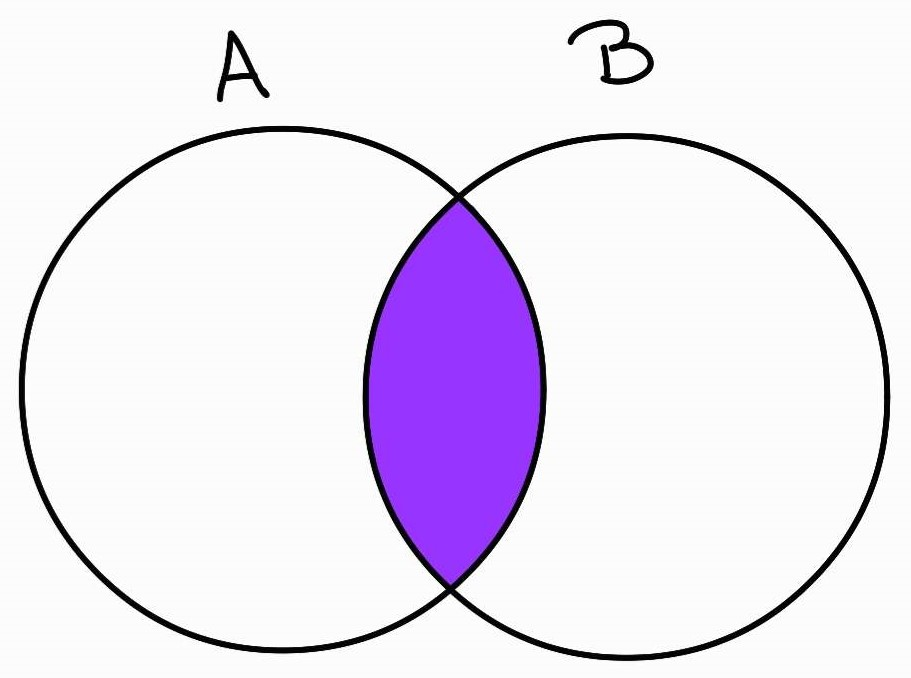
\includegraphics[width=0.4\linewidth]{innerjoin.jpg}
\caption{Diagrama de Venn de INNER JOIN}
\end{figure}
\item \textcolor{blue}{LEFT JOIN}: Devuelve todos los registros de la tabla izquierda y solo los registros coincidentes de la tabla derecha. Tanto en el \textcolor{blue}{LEFT JOIN} como el \textcolor{blue}{RIGHT JOIN} van a mostrar valores nulos. Si hace el cruce con columnas que tienen valores nulos, no cruza esos valores.
\begin{figure}[H] 
\centering 
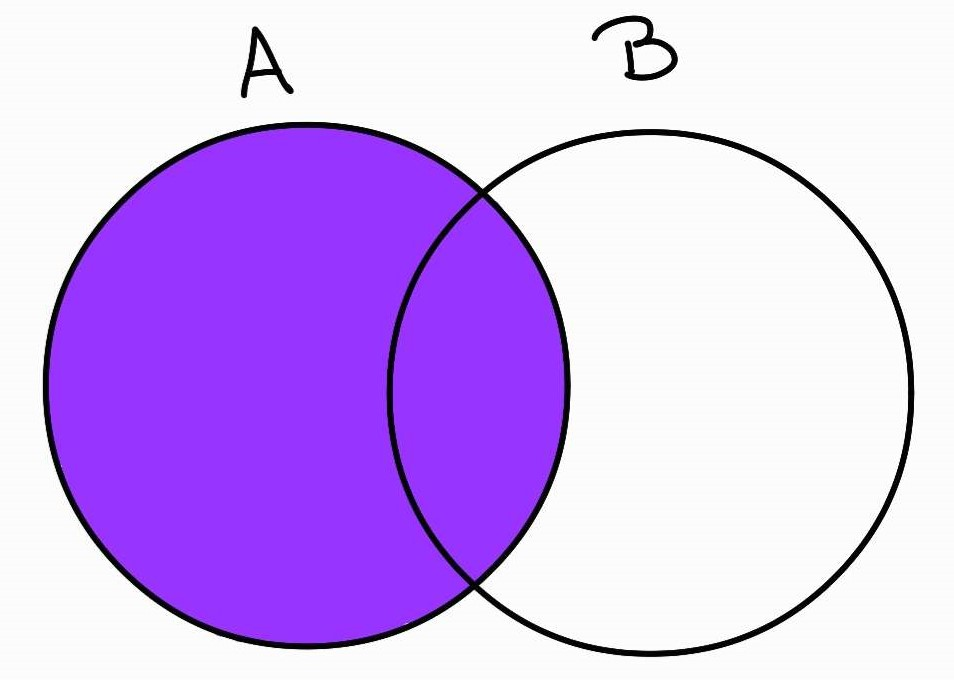
\includegraphics[width=0.4\linewidth]{leftjoin.jpg}
\caption{Diagrama de Venn de LEFT JOIN}
\end{figure}
\item \textcolor{blue}{RIGHT JOIN}: Devuelve todos los registros de la segunda tabla y solo los coincidentes de la primera tabla.
\begin{figure}[H] 
\centering 
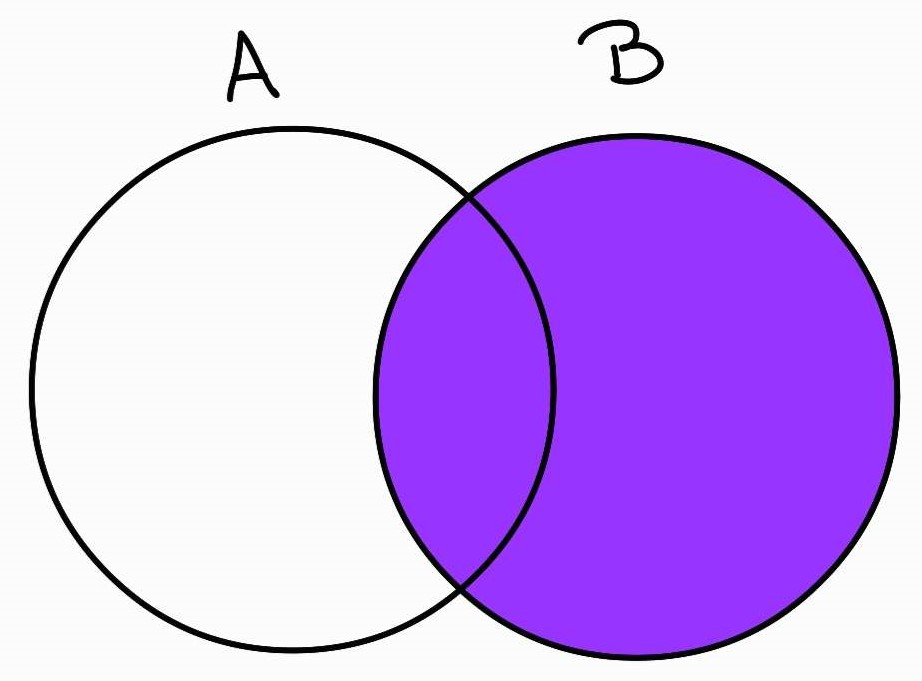
\includegraphics[width=0.4\linewidth]{rightjoin.jpg}
\caption{Diagrama de Venn de RIGHT JOIN}
\end{figure}
\item \textcolor{blue}{FULL JOIN}: Une todos los registros de las dos tablas, sean coincidentes o no.
\begin{figure}[H] 
\centering 
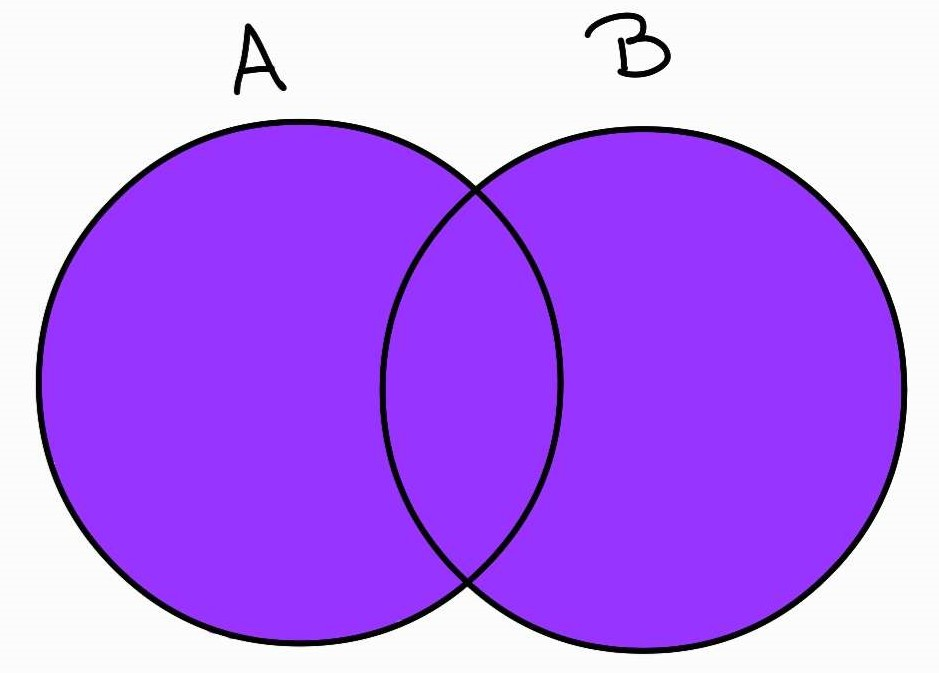
\includegraphics[width=0.4\linewidth]{fulljoin.jpg}
\caption{Diagrama de Venn de FULL JOIN}
\end{figure}
\item \textcolor{blue}{CROSS JOIN}: Combina cada uno de los registros de una tabla con los registros de la otra. No se hace sobre una clave, es decir, no va el \textcolor{blue}{ON}. La tabla resultante tendrá un número de filas igual al producto entre los números de filas de cada tabla, repitiéndose los datos de estas. Debido a esto, ocupa más recursos.
\end{enumerate}
%
%	CAPITULO
\chapter{Terminal Windows}
%	SECCION
\section{Comandos comunes}
\begin{enumerate}
	\item $\setminus$d tabla: muestra información de una tabla y los tipos de datos de cada columna.
	\item $\setminus$c base-de-datos: conectarse a una base de datos.
	\item $\setminus$dt: da una lista de todas las bases de datos.
    \item $\setminus$q: salir de la terminal.
    \item nom-programa version: verifica la versión instalada del programa en el sistema.
    \item clear: limpia la pantalla.
\end{enumerate}
%
%	CAPITULO
\chapter{Excel y Google Sheets}
%\textcolor{Green}{}
%	SECCION
\section{Notas previas...}
\begin{itemize}
\item Algunas funciones de Excel son parecidas a las de Google Sheets.
\item En Google Sheets se usan ; y en Excel ,.
\item Para los rangos se usa C:C, por ejemplo: =MAX(A3:A9).
\end{itemize}
%	SECCION
\section{Comandos básicos}
La sintaxis de una función en Excel y Google Sheets es =NOM-FUNCION(argumento1; argumento2;...), donde los argumentos son los valores que se usan como entrada para la función. \\
Se puede definir la hoja de cálculo con 'nom-hoja'!rango, por ejemplo: =CONTAR.SI('hoja 1'!G:G). En este ejemplo toma toda la columna G de la hoja 1.
%	SECCION
\section{Limpieza, orden y transformación de datos}
%	SUBSECCION
\subsection{Filtrado}
=FILTRAR(rango; fila-o-col = filtro;``"): Devolverá todos los registros del rango, y sin no hay devuelve una cadena vacía (``").
Se pueden crear filtros en Excel: Datos $>$ Filtro.
%	SUBSECCION
\subsection{Orden}
Para ordenar datos en hojas de cálculo, se debe seleccionar Datos $>$ Ordenar. También se puede hacer mediante la función =ORDENAR(). \\
En el siguiente comando, FALSO (o -1 en Excel) indica que el orden es descendiente. Por otro lado, VERDADERO (o 1 en Excel) señala orden ascendente.
=ORDENAR(rango-para-ordenar;segun-columna;FALSO) \\
\\
Usando =ORDENARPOR(): \\
=ORDENARPOR(rango;col-1; FALSO; col-2;VERDADERO)
%	SUBSECCION
\subsection{Quitar duplicados}
Para quitar duplicados en Excel: Datos $>$ Quitar espacios duplicados
%	SUBSECCION
\subsection{Funciones lógicas}
Las funciones lógicas utilizadas en Excel y Google Sheets son:
\begin{itemize}
\item Y(expresion1;expresion2;...)
\item O(expresion1;expresion2;...)
\item NO(valor-logico)
\item =SI(expresion;valor-si-verdadero;valor-si-falso)
\item =SI.ERROR(valor;valor-si-error)
\end{itemize}
%	SUBSECCCION
\subsection{Manipulación de strings}
\begin{enumerate}
\item =ESPACIOS(valores): Elimina espacios del texto.
\item =MAYUSC(celda): Cambia de minúscula a mayúscula.
\item =MINUSC(celda): Cambia de mayúscula a minúscula.
\item =NOMPROPIO(celda): Cambia a nombre propio.
\item =CONCATENAR(): Une dos o más cadenas de texto en una celda.
\item =ENCONTRAR(): Busca una cadena de texto y devuelve su posición.
\item =DERECHA(): Devuelve el número de caracteres iniciando desde la derecha.
\item =IZQUIERDA(): Devuelve el número de caracteres iniciando desde la izquierda.
\item =EXTRAE(): Devuelve un número específico de caracteres de una posición.
\item =LARGO(): Devuelve la longitud de una cadena de texto.
\item =REEMPLAZAR(): Reemplaza una cadena de texto por otra en una celda.
\end{enumerate}
%	SUBSECCION
\subsection{Formatos de fechas}
\begin{enumerate}
\item =HOY(): Devuelve la fecha actual.
\item =AHORA(): Devuelve fecha y hora actual.
\item =FECHA(): Crea una fecha. Ej: =FECHA(2023,6,10).
\item =DIAS360(): Calcula el número de días entre dos fechas en un año de 365 días.
\item =DIAS.LAB(): Calcula el número de días laborales entre dos fechas.
\item =DIAS(): Calcula el número de días entre dos fechas.
\item =MES(): Devuelve el número de mes de una fecha.
\item =AÑO(): Devuelve el año de una fecha.
\item =DIASEM(): Devuelve el número de día de la semana de 1 a 7 para una fecha.
\item =DIAS.LAB.INTL(): Calcula el número de días laborales entre dos fechas usando una definición personalizada de días laborales.
\item =FIN.MES(): Devuelve la fecha del último día del mes antes o después de un número determinado de mesas.
\end{enumerate}
%	SUBSECCION
\subsection{BURSCARV y BURSCARH}
Para relacionar tablas y buscar datos de una tabla a partir de una clave de búsqueda, se usan los comandos BUSCARV y BUSCARH. La principal diferencia entre ellos es que BUSCARV solo realiza la búsqueda en una columna, mientras que BUSCARH lo hace con las filas. \\
Si se escribe FALSO, la coincidencia será exacta. Si se escribe VERDADERO, la coincidencia será cercana. En Excel 1 es verdadero y 0 es falso: \\
=BUSCARV(valor-buscado; rango-de-busqueda; num-para-indicar-col-de-busqueda; FALSO)
%	SUBSECCION
\subsection{Formato de datos}
Se usa la función =CONVERTIR() se usa para transformar un número de un sistema de medición a otro. \\
=CONVERTIR(num-a-convertir;unidad-del-num;unidad-resultado) \\
%	SUBSECCION
\subsection{Formato condicional}
El formato condicional es una herramienta que se utiliza para identificar tendencias resaltándolas con colores. Se le añade una condición para que cambie el aspecto de la celda.


Se puede aplicar el formato condicional de la siguiente forma: \\
Excel: Se debe seleccionar el rango de celdas donde se quiera aplicar el formato $>$ Inicio $>$ Formato condicional $>$ Reglas para resaltar celdas. \\
Google Sheets: Se debe seleccionar el rango de celdas donde se quiera aplicar el formato $>$ Formato $>$ Formato condicional.
%	SECCION
\section{Análisis y visualización}
%	SUBSECCION
\subsection{Cálculos matemáticos básicos}
\begin{enumerate}
\item =SUMA(rango)
\item =PROMEDIO(rango)
\item =MIN(rango)
\item =MAX(rango)
\item =RESIDUO(): Da como resultado el resto cuando al dividir dos números.
\item =CONTAR.SI(rango; ''criterio"): Cuenta el número de celdas que cumplen con un criterio.
\item =SUMAR.SI(rango; ''criterio"): Suma los valores de un rango si cumplen con el criterio.
\item =SUMAPRODUCTO(matriz1;matriz2;...): Multiplica las matrices y muestra el resultado de la suma de esos productos.
\end{enumerate}
%	SUBSECCION
\subsection{Cálculos con múltiples criterios}
\begin{enumerate}
\item =SUMAR.SI.CONJUNTO(rango-suma;rango-criterio1;criterio1;rango-criterio2;criterio2;...)
\item =CONTAR.SI.CONJUNTO(rango-criterio1;criterio1;rango-criterio2;criterio2;...)
\item =MAX.SI.CONJUNTO(rango-max;rango1;criterio1;rango2;criterio2;...)
\end{enumerate}
%	SUBSECCION
\subsection{Tablas dinámicas}
Una tabla dinámica o Pivot Table es una tabla que resume, calcula y analiza datos para observar tendencias entre ellos. \\
Para crear una tabla dinámica tanto en Excel como en Google Sheets, se debe seleccionar Insertar $>$ Tabla dinámica, luego seleccionar los datos preferentemente limpios y con columnas.
%	SUBSECCION
\subsection{Creación de gráficos}
Para crear un gráfico tanto en Excel como en Google Sheets, se debe seleccionar Insertar $>$ Gráfico. Se puede personalizar cambiando los colores, dándole nombre a los ejes y variar el tipo de gráfico.
%	SECCION
\section{Importación de datos}
Si se desea importar datos de otras hojas de cálculo: \\
Excel: Datos$>$Obtener datos$>$ Desde archivo $>$ Desde libro$>$ seleccionar archivo $>$ Importar$>$ seleccionar en el navegador la hoja de trabajo que e quiere importar $>$ Cargar o Transformar datos. \\
Google Sheets: =IMPORTRANGE(), el cual permite especificar un rango de celdas en la otra hoja de cálculo para duplicarlo en la hoja que se esté trabajando.
%	SECCION
\section{Errores}
\begin{itemize}
\item $\#$DIV/0!: Fórmula que intenta dividir por cero un valor en una celda o por una celda vacía. Se soluciona con: =SI.ERROR(valor; valor-si-hay-error).
\item $\#$ERROR!: Error que solo devuelve Google Sheets. Señala que la fórmula no se puede interpretar tal como se ingresa, es decir, hay un error en la fórmula.
\item $\#$N/A: Indica que la hoja de cálculo no puede encontrar los datos de la fórmula. Ocurren generalmente cuando se usa la función =BUSCARV().
\item $\#$NAME? o $\#$NOMBRE?: ocurre cuando el nombre de una fórmula no se reconoce.
\item $\#$NUM!: Señala que el cálculo de una fórmula no se puede realizar según lo especificado por los datos, como por ejemplo una fecha negativa.
\item $\#$VALUE!: Señala un problema con la fórmula o con las celdas con las que hace referencia.
\item $\#$REF!: Aparece cuando las celdas de una fórmula se han eliminado.
\end{itemize}
%
%	CAPITULO
\chapter{Tableau Public}
Tableau Public es una plataforma para crear y compartir visualizaciones de datos en línea.

Una visualización de datos es una representación gráfica de los mismos para comunicar información de manera efectiva. Se usa principalmente para identificar patrones que pueden ser difíciles de detectar en una tabla de datos, explorar datos, comunicar información, ayudar a tomar decisiones informadas, hacer seguimiento a procesos, identificar problemas de procesos y más.

%	SECCION
\section{Creación de visualizaciones}
%	SUBSECCION
\subsection{Importación de datos y conexiones}
Para importar datos, se pueden cargar archivos desde el equipo o conectarse con Google Drive. Si se desean agregar más de un archivo, se debe seleccionar el signo + al lado de Conexiones.
\begin{figure}[H] 
	\centering 
	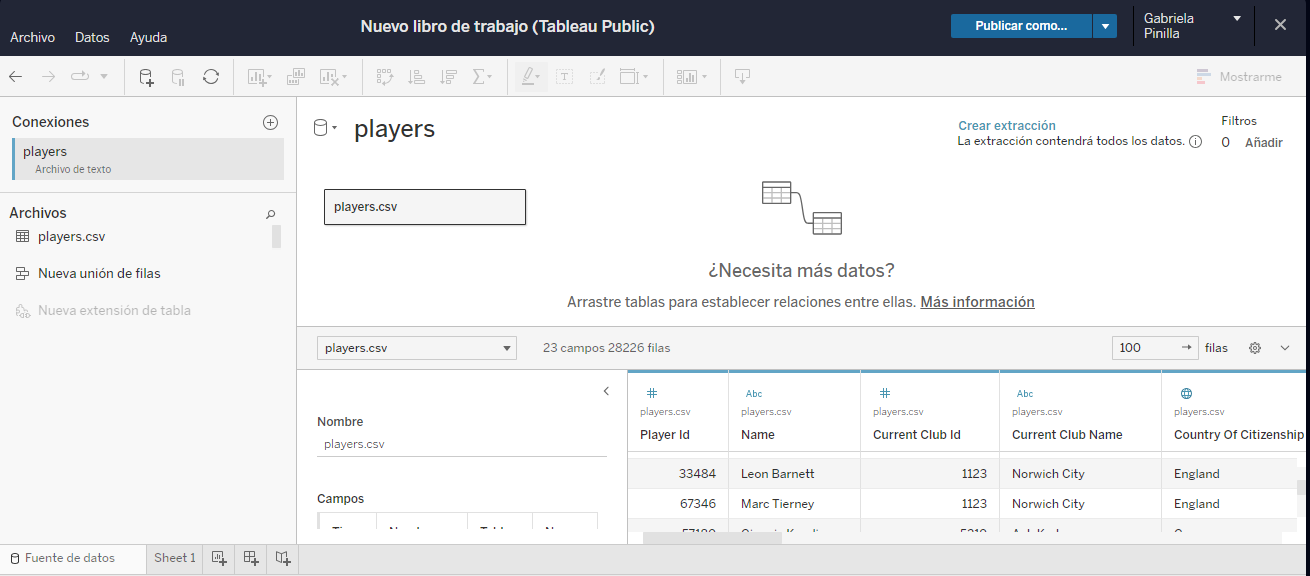
\includegraphics[width=1.0\linewidth]{foto1.png}
	\caption{Fuente de datos}
\end{figure}
En la esquina inferior derecha se muestran los datos en una tabla. Hacia la izquierda en Conexiones, se muestran las fuentes de los datos, los cuales se pueden conectar unos con otros arrastrándolos hacia el panel que dice ¿Necesita más datos?, quedando de la siguiente forma:
\begin{figure}[H] 
	\centering 
	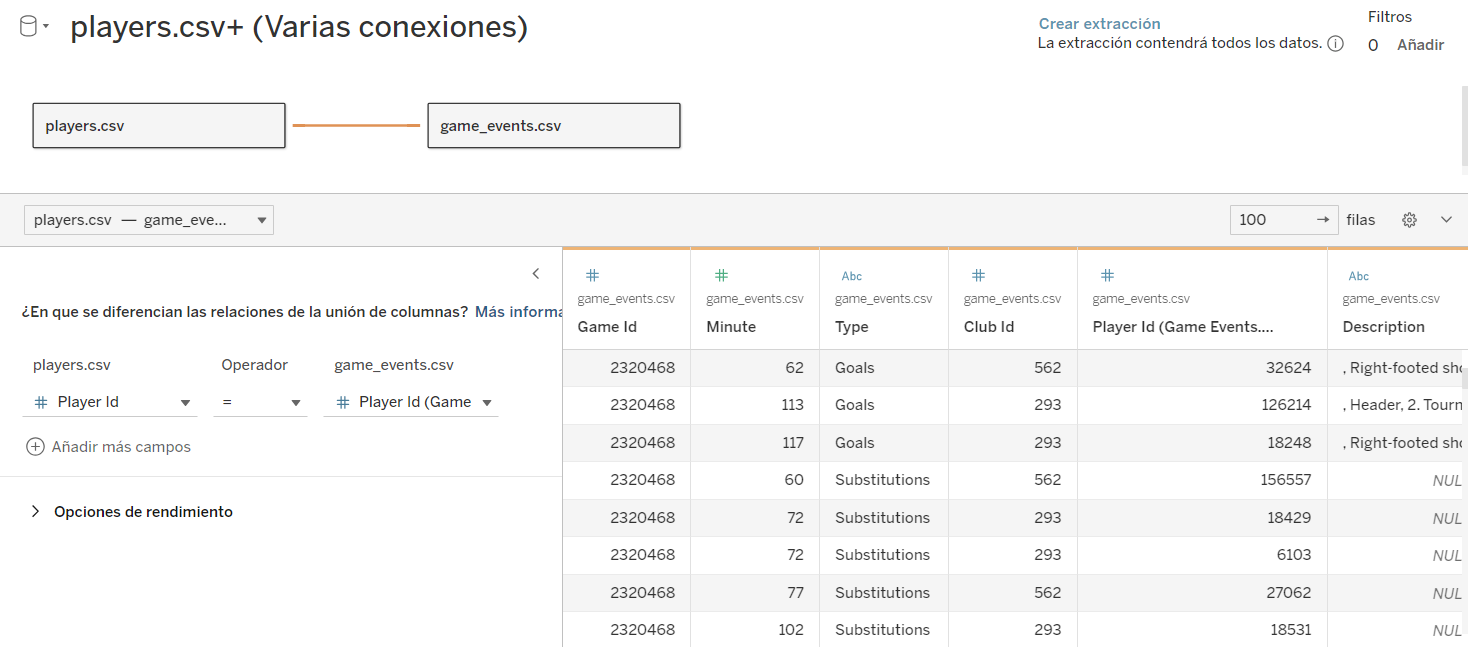
\includegraphics[width=1.0\linewidth]{foto2.png}
	\caption{Campos en común}
\end{figure}
Tableau detecta si hay un campo en común entre ambos archivos csv la cual muestra bajo la conexión de las fuentes.
%	SUBSECCION
\subsection{Campos calculados}
Desde la misma hoja de Fuentes de datos se pueden realizar cálculos en las tablas. Para hacerlo, se debe seleccionar la tabla, luego la flecha de la columna en la que se desea crear un campo calculado, $>$ Crear $>$ Campo calculado...

Se le puede asignar un nombre al campo calculado y escribir la fórmula para calcular los valores del campo seleccionado con los nombres de los campos entre paréntesis de corchetes. Ejemplo: [Campo 1]*5.

En Tableau existen funciones básicas que se pueden utilizar para las fórmulas de los campos calculados:
\begin{enumerate}
	\item CONTAINS: Retorna verdadero si una cadena contiene una subcadena. Ejemplo: CONTAINS("Hola a todos","todos"), devolverá verdadero.
	\item LTRIM: Elimina los espacios en blanco del lado izquierdo de una cadena. Ejemplo: LTRIM("    Hola"), devuelve "Hola".
	\item TRIM: Elimina los espacios en blanco de ambos lados de una cadena. Ejemplo: TRIM("  Hola  "), retorna "Hola"
	\item SPLIT(): Divide un campo según un separador especificado y un token. Ejemplo: SPLIT([Nombre completo], ' ', 2), en el caso de que el nombre sea Juan Soto, devolverá Soto. Si el token es 1, devolverá Juan.
	\item LEN: Devuelve el largo de una cadena de texto. Ejemplo: LEN("Hola a todos"), devuelve 12.
	\item LEFT: Devuelve los primeros caracteres de una cadena según una cantidad especificada. Ejemplo: LEFT("Hola a todos", 4), devuelve "Hola".
	\item RIGHT: Devuelve los caracteres iniciando desde la derecha hacia la izquierda. Ejemplo: RIGHT("Hola a todos", 5), devuelve "todos".
	\item LOWER: Convierte el texto en minúsculas. Ejemplo: LOWER("HOLA"), devuelve hola.
	\item UPPER: Convierte el texto en mayúsculas. Ejemplo: UPPER("hola"), devuelve "HOLA".
	\item MAX: Retorna el valor máximo de una expresión. Ejemplo: MAX([Ventas]), retornará el valor máximo de la columna Ventas.
	\item REPLACE: Reemplaza una subcadena de texo por otra. Ejemplo: REPLACE("Hola a todos", "todos", "todas las mujeres presentes aquí"), devuelve "Hola a todas las mujeres presentes aquí".
	\item COUNT: Muestra la cantidad de filas de un campo. Ejemplo: COUNT([Libros]), devolverá la cantidad de libros.
	\item CEILING: Devuelve el número entero más pequeño mayor o igual que un número especificado. Ejemplo: CEILING(5,13), devuelve 5.
	\item FLOOR: Devuelve el número entero más grande menor o igual que un número especificado. Ejemplo: FLOOR(5,16), devuelve 3.
	\item ROUND: Redondea un número con decimales especificados. Ejemplo: ROUND("5,1634546", 2), devuelve 5,16.
	\item LOG: Devuelve el logaritmo en base e de un número.
	\item DATE: Devuelve la fecha. Ejemplo: DATE(01/05/2023 00:00:00), devuelve 01/05/2023.
	\item DATEDIFF: Devuelve la diferencia entre dos fechas. Ejemplo: DATEDIFF(01/09/2023, 10/09/2023, DAY), devolverá la cantidad de días entre ambas fechas.
	\item DATENAME: Devuelve el nombre de un mes, día de la semana o del año.
	\item DATEPART: Devuelve una parte específica de una fecha. Ejemplo: DATEPART(01/09/2023, YEAR), devolverá 2023.
\end{enumerate}

%	SUBSECCION
\subsection{Conceptos y elementos de Tableau}
Al momento de crear un dashboard, se debe tener en consideración ciertos términos y elementos de la plataforma.

Una hoja de trabajo es un espacio donde se puede construir la visualización de datos. Sus elementos principales son:
\begin{itemize}
	\item Filas y columnas: aquí es donde el usuario puede arrastrar los campos de datos para definir las dimensiones y medidas de la visualización.
	\item Dimensiones y medidas: en el panel de datos se pueden encontrar los datos divididos por una línea donde los de arriba representan las dimensiones y los de abajo las medidas. 
	\begin{itemize}
		\item Las dimensiones son los datos categóricos. Su fin es clasificar la información. Los tipos de dimensiones son: fechas, cadenas de texto, booleanos (verdadero o falso) y rol geográfico. Ejemplo: género, estado civil.
		\item Las medidas son datos de origen cuantitativos que asignan valores a las dimensiones. Los tipos de medidas son: números y rol geográfico (latitud y longitud). Ejemplo: cantidad de habitantes.
	\end{itemize}
	En este mismo panel, se encuentran datos de color azules, los cuales corresponden a datos discretos. Se tratan como finitos. Por el contrario, los verdes son datos continuos. Se tratan como un intervalo infinito.
	\item Marcas: en la tarjeta de marcas se configura la forma en que las dimensiones y medidas serán representadas. Sus elementos son: Tipo de marca: el cual indica la forma en la que se van a graficar los datos; Color: permite cambiar los colores de la visualización; Tamaño: varía el tamaño de la visualización; Texto: permite definir el texto de la etiqueta a mostrar en la gráfica; Detalle: permite agregar información a las marcas; Descripción emergente: permite que al pasar el mouse por una marca se muestre una descripción emergente con información.
	\begin{figure}[H] 
		\centering 
		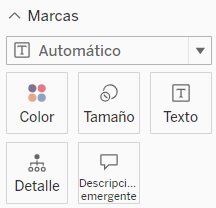
\includegraphics[width=0.3\linewidth]{marcas.png}
		\caption{Tarjeta de marcas}
	\end{figure}
	\item Filtros: aplica filtros al arrastrar los campos a este estante.
	\item Páginas: se pueden arrastrar campos para crear páginas en la visualización.
\end{itemize}

%	SUBSECCION
\subsection{Filtros}
\begin{enumerate}
	\item Filtros de extracción: se usan para limitar el conjunto de datos desde la Fuente de datos. Al aplicarlo, se abrirá una ventana para añadir los filtros que se deseen.
	\begin{figure}[H] 
		\centering 
		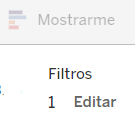
\includegraphics[width=0.2\linewidth]{filtro1.png}
		\caption{Filtro de extracción}
	\end{figure}
	\item Filtros de contexto: se usan para definir un contexto específico en los cálculos. En lugar de aplicar un filtro para el conjunto de datos, crea un subconjunto de datos para hacer cálculos. Para crear un filtro de contexto, se debe arrastrar un campo al estante de filtros en la hoja de trabajo, luego seleccionar la flecha de la cápsula del campo y seleccionar Añadir a contexto.
	\begin{figure}[H] 
		\centering 
		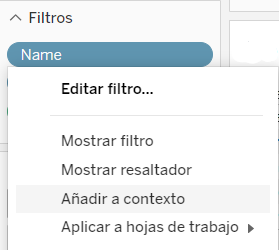
\includegraphics[width=0.3\linewidth]{filtro2.png}
		\caption{Filtro de contexto}
	\end{figure}
	\item Filtro de dimensión: se usan para filtrar datos de dimensiones discretas.
	\begin{figure}[H] 
		\centering 
		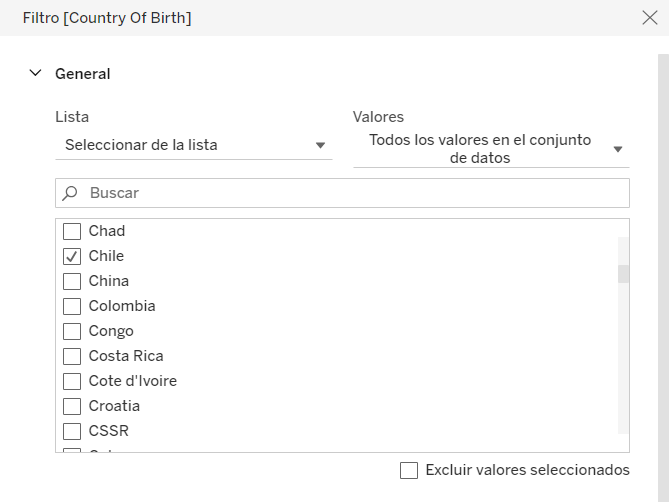
\includegraphics[width=0.6\linewidth]{filtro3.png}
		\caption{Filtro de dimensión}
	\end{figure}
	\item Filtro de medida: se usan para filtrar datos en función de una medida continua.
	\begin{figure}[H] 
		\centering 
		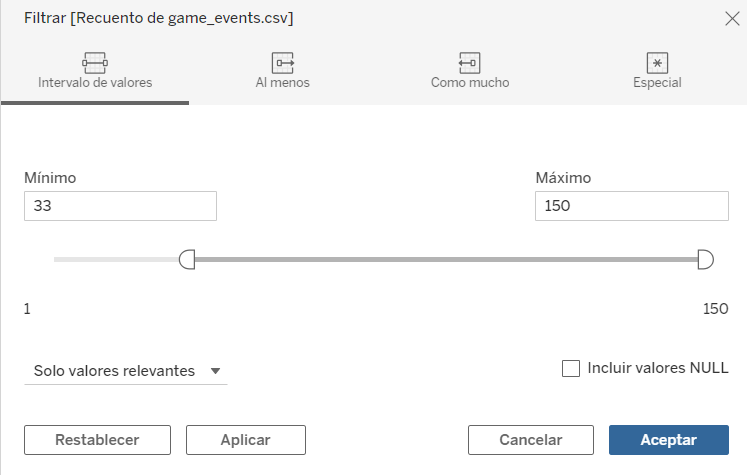
\includegraphics[width=0.5\linewidth]{filtro4.png}
		\caption{Filtro de medida}
	\end{figure}
	\item Filtro en gráfico: se pueden filtrar datos en un gráfico.
\end{enumerate}

%	SECCION
\section{Creación de visualizaciones básicas}
La creación de visualizaciones en Tableau se hace arrastrando las tablas de datos hacia los estantes de filas, columnas, marcas y filtros.

En el siguiente ejemplo se utilizó la base de datos del siguiente enlace de Kaggle \url{Uhttps://www.kaggle.com/datasets/ishikajohari/shazam-global-top-200-per-week?resource=download}, el cual muestra datos del top 200 por semana de Shazam, una aplicación para identificar música y otros desde los dispositivos móviles.

Con la base de datos de la primera semana (Week1 -22-Jul-to-28-Jul-2023.csv), se construyó la siguiente tabla:
\begin{figure}[H] 
	\centering 
	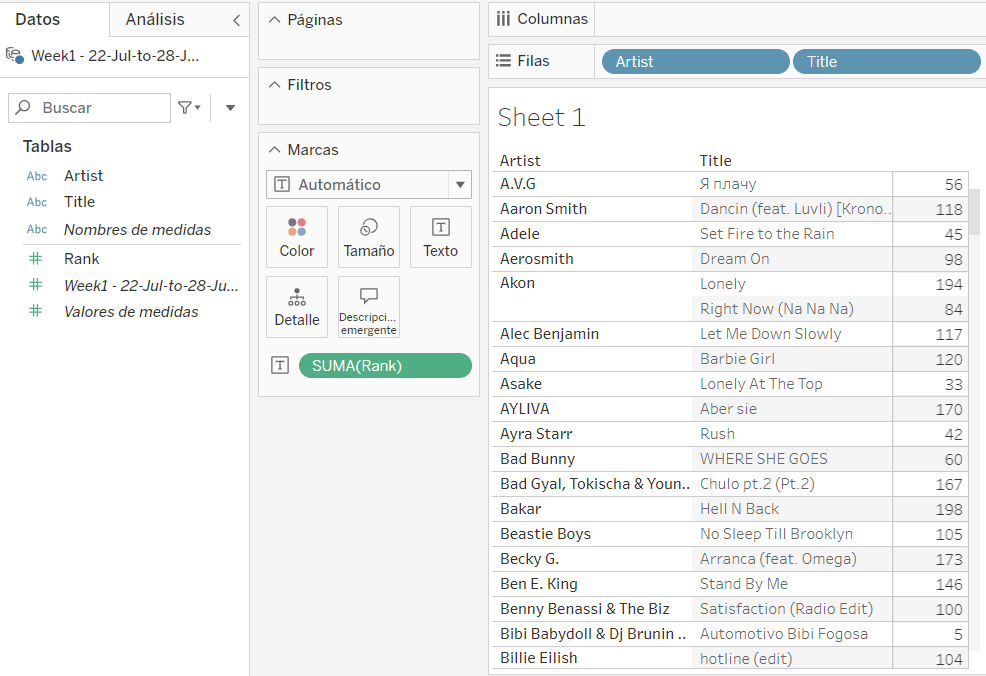
\includegraphics[width=0.9\linewidth]{tabla1.png}
	\caption{Tabla de datos creada en Tableau}
\end{figure}
En el estante de filas se añadieron Artist (dimensión) y Title (dimensión), mientras que Rank (medida) se añadió a Texto en Marcas, mostrando en la tabla el rankin de la canción y al artista a quien le pertenece. Por defecto, Tableau añade una función de agregación, que en el caso del ejemplo es SUMA, sin embargo, como se trata de un rankin, solo corresponde a un número y no a una suma.

En la misma tabla, se pueden ordenar los datos por el rankin, como de mayor a menor, sin embargo, al tener dos dimensiones en las filas no mostrará cuál canción es menos escuchada en el rankin, sino que mostrará un conjunto de canciones con su rankin perteneciente al mismo artista.
\begin{figure}[H] 
	\centering 
	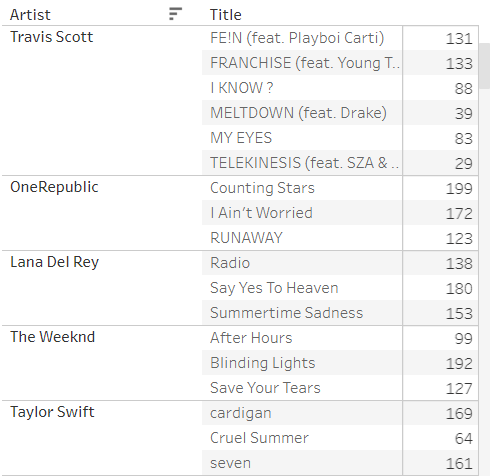
\includegraphics[width=0.5\linewidth]{tabla2.png}
	\caption{Tabla de datos creada en Tableau}
\end{figure}
Para descubrir cuál es la canción menos escuchada, se debe dejar solo una dimensión en filas, como Title, y luego ordenarlas. Si se quiere saber cuál es el artista menos escuchado, se debe hacer lo mismo con la dimensión Artist.
\begin{figure}[H] 
	\centering 
	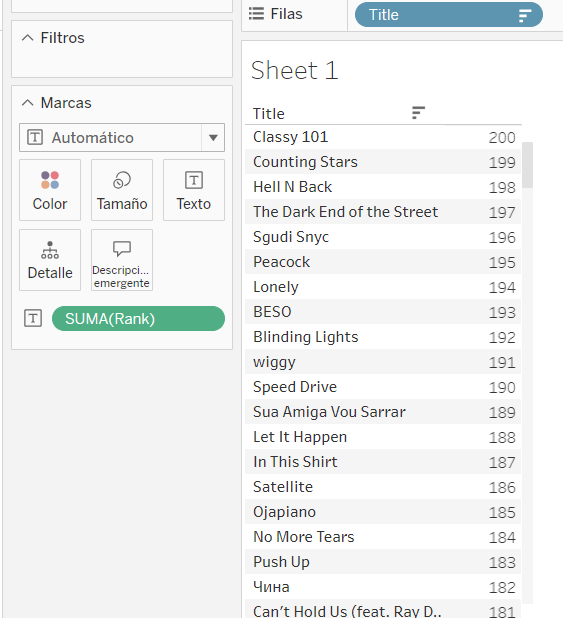
\includegraphics[width=0.7\linewidth]{tabla3.png}
	\caption{Tabla de datos creada en Tableau}
\end{figure}
También, se puede modificar la medida Rank para que cuente la cantidad de canciones con la que los artistas aparecen en el rankin.
\begin{figure}[H] 
	\centering 
	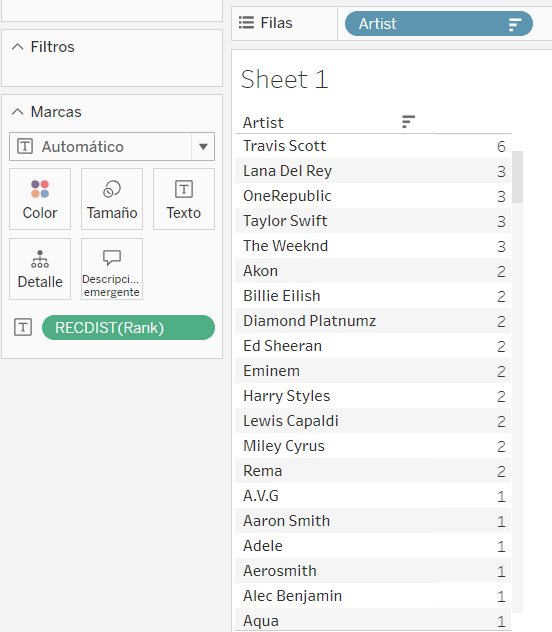
\includegraphics[width=0.7\linewidth]{tabla4.png}
	\caption{Tabla de datos creada en Tableau}
\end{figure}


Para el siguiente ejemplo, se tomó la base de datos mensual de las 50 principales cuentas de redes sociales de
\url{https://www.kaggle.com/datasets/amyrmahdy/monthly-top-50-social-media-accounts-dataset}.

Con al base de datos del top 50 de Youtube (youtube$\_$top$\_$50$\_$2023-07-03), se construyó la siguiente visualización:
\begin{figure}[H] 
	\centering 
	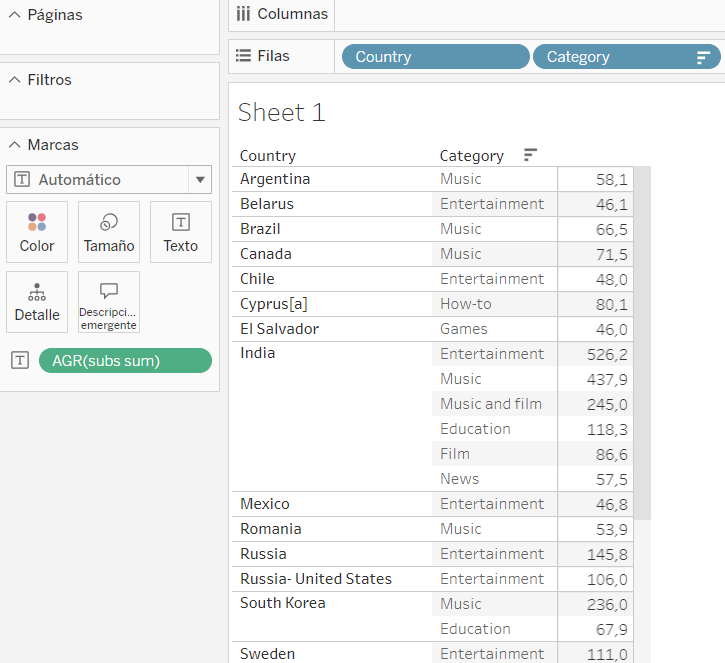
\includegraphics[width=0.7\linewidth]{tabla5.png}
	\caption{Tabla de datos creada en Tableau}
\end{figure}
Esta tabla muestra la categoría (Category) de cada país (Country) ordenado de mayor a menor por la suma de los subscriptores (subs sum) de cada categoría. Esta suma se realizó en el campo calculado de la Fuente de datos con el código SUM([Subscribers (millions)]).

Sin embargo, estos datos también se pueden representar de forma geoespacial por medio de un mapa.
\begin{figure}[H] 
	\centering 
	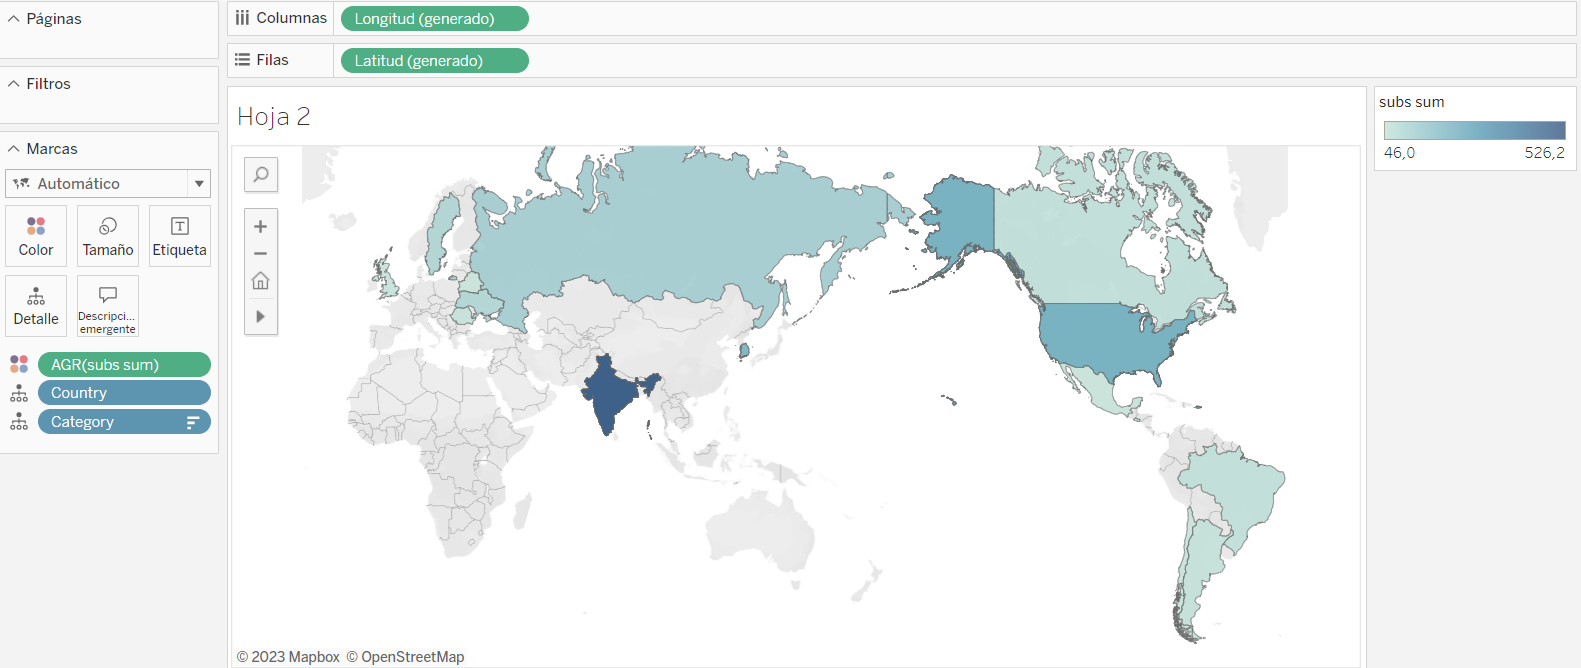
\includegraphics[width=0.9\linewidth]{mapa1.png}
	\caption{}
\end{figure}
Ordenando los subscriptores de forma descendente, se obtiene un mapa que muestra la categoría con más subscriptores en los países, donde el color azul indica un número más alto que el color celeste claro.

Para hacer esto, se agregó la tabla de subscriptores a la marca de Color, de esta forma Tableau puede hacer un mapa de calor indicando qué países tienen una mayor cantidad de subscriptores. La categoría y el país se arrastraron hacia la marca de Detalles, por lo que al pasar el mouse por encima de alguno de estos países mostrará el nombre del país, la categoría y la cantidad de subscriptores. La latitud y longitud en filas y columnas se generó a partir de la tabla Country.

%	SECCION
\section{Diseño y personalización de paneles}
Al graficar, se debe tener en consideración el tipo de datos que presenta la base de datos dado que no todos los gráficos sirven para representar cualquier tipo de datos.

Para elegir un gráfico que va a representar un conjunto de datos, es importante saber qué es lo que se quiere mostrar con la visualización, conocer los tipos de gráficos y saber cuál es la audiencia a quienes se les va a presentar.

A continuación, se presentan algunos tipos de gráficos:
\begin{enumerate}
	\item Gráfico de columnas: Compara categorías usando barras verticales.
	\item Gráfico de barras: Compara categorías usando barras horizontales.
	\item Gráfico circular: Proporciona las categorías en relación al total.
	\item Gráfico de líneas: Muestra las tendencias a lo largo del tiempo usando líneas.
	\item Gráfico de área: Muestra las tendencias a lo largo del tiempo usando un área sombreada bajo la línea.
	\item Gráfico de dispersión: Relaciona dos conjuntos de datos usando puntos.
	\item Gráfico de burbujas: Relaciona dos conjuntos de datos usando burbujas de diferentes tamaños para mostrar la magnitud de un tercer conjunto de datos.
	\item Histograma: Distribuye los datos en un rango continuo.
	\item Gráfico de radar: Expone los datos en un formato circular con categorías que se extienden radialmente.
\end{enumerate}

%	SUBSECCION
\subsection{Funciones de agregación}
Las funciones de agregación son una funciones que operan sobre un conjunto de datos que devuelven un único valor. Se pueden obtener el promedio de un conjunto, máximo, mínimo, recuento o suma.

Las funciones de agregación más comunes en Tableau son:
\begin{itemize}
	\item Promedio
	\item Suma
	\item Promedio o media
	\item Mediana
	\item Recuento: devuelve la cantidad de filas. Ejemplo: Rec(a,a,b,b)=4.
	\item Recuento (distintos): devuelve la cantidad de valores distintos de una columna. Ejemplo: RecDis(a,a,b,b)=2.
	\item Máximo y mínimo
	\item Desviación estándar y desviación estándar poblacional
	\item Varianza y varianza poblacional
\end{itemize}
Para agregar una función de agregación, se debe seleccionar Medida $>$ Suma, Promedio, Mediana...

Por defecto, Tableau agrega la suma para medidas numéricas y el recuento para las no numéricas.
%	SUBSECCION
\subsection{Funciones LOD}
Las funciones LOD (Level of Detail) en Tableau permite realizar cálculos en un nivel de detalle específico en los datos. Son útiles cuando se requiere realizar cálculos que no se pueden lograr con las funciones de agregación.

Tableau tiene tres tipos de funciones LOD:
\begin{enumerate}
	\item FIXED: permite definir un nivel de detalle específico para un cálculo. Ejemplo: Para calcular la suma de ventas por categoría: {FIXED [Categoria] : SUM([Ventas])}.
	\item INCLUDE: permite incluir un nivel de detalle específico a un cálculo sin afectar el nivel de detalle general de la visualización. Ejemplo: Para calcular la suma de ventas por categorías e incluir la ciudad: {INCLUDE [Categoria],[Ciudad] : SUM([Ventas])}.
	\item EXCLUDE: permite excluir un nivel de detalle específico a un cálculo sin afectar el nivel de detalle general de la visualización.
\end{enumerate}

%	SECCION
\section{Dashboards}
Un dashboard consiste en una pantalla que presenta una colección de visualizaciones que resumen información importante.

Uno de los propósitos de un dashboard es monitorear el rendimiento de un a empresa por medio de KPI, presentando la información de forma clara para que el público pueda entenderla.

Un KPI (Key Performance Indicator o Indicador Clave de Rendimiento) es una medida que evalúa el rendimiento de una empresa o proceso con respecto al objetivo empresarial. Los KPI siguen la metodología S.M.A.R.T., un acrónimo que explican las características básicas de un objetivo SMART. Estos deben ser específicos (Specific), medibles (Measurable), alcanzables (Attainable), realistas (Realistic) y con un tiempo límite (Time).

Ejemplos de métricas que se pueden usar para los KPI:
\begin{itemize}
	\item ROI
	\item Número de clientes nuevos
	\item Tasa de satisfacción
	\item Tasa de rotación del personal
	\item Porcentaje de clics en una página web
	\item Cantidad de carritos de compras abandonados
	\item IPC
\end{itemize}
%	SUBSECCION
\subsection{Creación de un dashboard}
Para crear un dashboard, se debe seleccionar el icono de Nuevo dashboard.

Luego, arrastrar las vistas desde la lista de Hojas hacia el dashboard.

%
%	CAPITULO
\chapter{Python}
% \texttt{\textcolor{blue}{}}
%	SECCION
\section{Notas previas...}
\begin{enumerate}
	\item Python es un lenguaje de programación orientado a objetos de alto nivel.
	\item Los tipos de datos en Python son int (números enteros), float (decimales), string (cadenas de texto) y booleanos.
	\item Los strings se escriben entre comillas simples o dobles.
	\item Los comentarios se hacen con el numeral ($\#$). Los comentarios que contengan más de una línea se hacen en un bloque de tres comillas simples:
	\begin{minted}[breaklines, breakanywhere]{Python}
# Esto es un comentario
		
'''
Esto
es un
comentario
'''
	\end{minted}
\end{enumerate}

%	SECCION
\section{Librerías}
En ciencia de datos, las librerías más usadas son NumPy, Matplotlib y Pandas.
%	SUBSECCION
\subsection{Importación de datos}
Para importar las librerías, se utiliza el comando \texttt{\textcolor{blue}{import}} y, usualmente, se le asigna un alias:
\begin{minted}[breaklines, breakanywhere]{Python}
import libreria as alias
\end{minted}
Si se quiere importar solo una función de una librería:
\begin{minted}[breaklines, breakanywhere]{Python}
from libreria import funcion as alias
\end{minted}
Ejemplo:
\begin{minted}[breaklines, breakanywhere]{Python}
# Funcion que genera un numero aleatorio entre 0 y 10
import random
num = random.randit(0, 10)
print('El numero es ', num)
\end{minted}


En Google Colaboratory, se importan los datos de drive con Pandas:
\begin{minted}[breaklines, breakanywhere]{Python}
from google.colab import drive
drive.mount('/content/drive')
\end{minted}
Luego, ir a Archivos $>$ Drive $>$ Copiar ruta de acceso. Se debe importar la librería Pandas con un alias:
\begin{minted}[breaklines, breakanywhere]{Python}
import pandas as pd
\end{minted}
Finalmente, para leer un archivo en formato csv:
\begin{minted}[breaklines, breakanywhere]{Python}
nom_ds = pd.read_csv('ruta-del-archivo.csv')
\end{minted}

%	SECCION
\section{Conceptos previos}
%	SUBSECCION
\subsection{Manipulación de strings}
Los strings son cadenas de textos que contienen una secuencia de caracteres, como palabras. Se definen usando comillas simples o dobles y se pueden realizar operaciones con ellas.

Para interactuar con el usuario, se usan los comandos \texttt{\textcolor{blue}{print}} y \texttt{\textcolor{blue}{input}}. El primero imprime un mensaje en pantalla, mientras que el segundo permite que el usuario ingrese datos.
\begin{minted}[breaklines, breakanywhere]{Python}
# Imprimir texto en pantalla
print('Hola mundo')
	
# Toma informacion y la puede guardar en una variable
nombre=input('Cual es tu nombre?')
	
# Sustituir variables en un string
print(f'Tu nombre es: {nombre}')

# Concatenacion
print('hola' + ' '+ 'mundo')
# salida: hola mundo
	
# Repeticion
print('Ja' * 4)
# salida: JaJaJaJa
\end{minted}


Para transformar un número a string:
\begin{minted}[breaklines, breakanywhere]{Python}
str(15)
# salida: 15
	
print('Quiero ' + str(15) + ' panes')
\end{minted}
Y de un string a número:
\begin{minted}[breaklines, breakanywhere]{Python}
edad = int(input('Cual es tu edad?'))
\end{minted}
Operaciones con strings:
\begin{minted}[breaklines, breakanywhere]{Python}
texto = 'Hola a todos'
# 1. lower(): convierte los caracteres a minusculas
texto_1 = texto.lower()
print(texto_1)
# salida: hola a todos
	
# 2. upper(): convierte los caracteres a mayusculas
texto_2 = texto.upper()
print(texto_2)
# salida: HOLA A TODOS
	
# 3. replace(sub, new_sub): reemplaza texto por uno nuevo
texto_3 = texto.replace('todos','Marta')
print(texto_3)
# salida: Hola a Marta
	
# 4. split(sep): divide una cadena en una lista con un separador
textonuevo = 'Hola,Josesa'
lista = textonuevo.split(',')
print(lista)
# salida: ['Hola', 'Josefa']
	
# 5. strip(): elimina los espacios en blanco al inicio y final de una cadena
otrotexto = '	Hola	'
texto_4 = otrotexto.strip()
print(texto_4)
# salida: Hola
\end{minted}

%	SUBSECCION
\subsection{Estructuras de datos}
Listas o arreglos: son secuencias de elementos ordenados por un índice, empezando por el 0.
\begin{minted}[breaklines, breakanywhere]{Python}
# Crear una lista
lista_1 = ['elemento0', 'elemento1', 'elemento2']
print(lista_1) # Imprime la lista

# Para acceder a los elementos de la lista:
print(lista_1[0])
# salida: elemento0
	
print(lista_1[2]) # o print(lista_1[-1])
# salida: elemento2
	
# Para agregar un elemento al final de la lista
lista_1.append('elemento3')
print(lista_1)
# salida: ['elemento0', 'elemento1', 'elemento2', 'elemento3']
	
# Para obtener la longitud
longitud = len(lista_1)
print(longitud)
# salida: 4
\end{minted}

Diccionarios: es una colección de par clave-valor. Su sintaxis es $\{clave: valor\}$:
\begin{minted}[breaklines, breakanywhere]{Python}
diccionario_1={'nombre':'Marcelo',
	'apellido':'Soto',
	'ciudad':'Santiago',
	'edad':38,
	'profesion':'Presidente'}

# Imprimir un valor
print({diccionario_1['profesion']})
# salida: Presidente
	
# Agregar un nuevo par clave-valor
diccionario_1['estado civil'] = 'Soltero'
\end{minted}

Tuplas: las tupla no se pueden modificar después de haber sido creada.
\begin{minted}[breaklines, breakanywhere]{Python}
tupla_1=('elemento0', 'elemento1', 'elemento3')
	
# Para que devuelva 'elemento0'
tupla_1[0]
\end{minted}

Set: no permite tener elementos repetidos. Guardará solo los datos que no se repiten.
\begin{minted}[breaklines, breakanywhere]{Python}
set_1 = {'banana', 'manzana', 'pera'}
\end{minted}

%	SECCION
\section{Limpieza, orden y transformación de datos}

%	SUBSECCION
\subsection{Bibliotecas}
Las bibliotecas que más se usan en Python para la ciencia de datos son Pandas, NumPy, Scikit-learn y Matplotlib.

NumPy se especializa en el cálculo y análisis de datos, la cual permite manejar datos de forma rápida por medio de los NumPy Arrays o ndarray, una estructura de datos que puede ser de una dimensión (vector), dos dimensiones (matriz), tres (cubo) o más.

Por lo general, se importa con el alias np:
\begin{minted}[breaklines, breakanywhere]{Python}
import numpy as np
\end{minted}
Por otro lado, la biblioteca Pandas permite manipular y analizar estructuras de datos. Se basa en NumPy y proporciona los siguientes tipos de datos:
\begin{enumerate}
	\item Series: Estructuras de una dimensión.
	\item DataFrame: Estructura de dos dimensiones.
	\item Panel: Estructura de tres dimensiones.
\end{enumerate}
Se importa bajo el alias de pd:
\begin{minted}[breaklines, breakanywhere]{Python}
import pandas as pd
\end{minted}


Scikit-learn es una biblioteca de aprendizaje automático que proporciona acceso a algoritmos comunes.
\\

Matplotlib se especializa en la generación de gráficos en dos dimensiones y personalización de estos. Se pueden crear diagramas de barras, mapas de calor, histogramas y más.

Por lo general, se importa con el alias plt:
\begin{minted}[breaklines, breakanywhere]{Python}
import matplotlib.pyplot as plt
\end{minted}

%	SUBSECCION
\subsection{NumPy Arrays}
Un NumPy Array se puede crear a partir de una lista usando el comando \texttt{\textcolor{blue}{np.array}}:
\begin{minted}[breaklines, breakanywhere]{Python}
# Arreglo 1d
a = np.array([1,2,3,4,5])
	
# Arreglo 2d
b = np.array([[3,4,5],
[4,3,2]])
\end{minted}
O por medio de \texttt{\textcolor{blue}{no.arrange}}, el cual crea un arreglo de una dimensión con valores del 0 a n:
\begin{minted}[breaklines, breakanywhere]{Python}
# Sintaxis
# a = np.arrange(inicio, fin-1,paso)
d = np.arrange(3,8,1)
\end{minted}

Propiedades:
\begin{minted}[breaklines, breakanywhere]{Python}
# Dimension del arreglo
arreglo.ndim
	
# Forma del arreglo (filas,columnas)
arreglo.shape
	
# Cantidad de datos en el arreglo
arreglo.size
\end{minted}

Para buscar valores en un arreglo, Python toma cada fila como un arreglo, donde el primero tendrá índice cero. Lo mismo ocurre con sus columnas, como se muestra a continuación:
\begin{minted}[breaklines, breakanywhere]{Python}
#       0  1  2
array([[1, 0, 3],  # indice 0
	[2, 6, 9],  # indice 1
	[4, 5, 8]]) # indice 2
\end{minted}
De esta forma, para seleccionar el número 6, se debe insertar \texttt{\textcolor{blue}{arreglo[1,1]}}.


Generación de números aleatorios:
\begin{minted}[breaklines, breakanywhere]{Python}
# Crea un arreglo de numeros aleatorios entre 0 y 1
a_1 = np.random.default_rng(n)
	
# Genera n valores aleatorios que siguen una distribucion normal.
normal(media, desv_estandar,n)

# Genera n numeros aleatorios entre el 0 y fin-1.
integers(fin-1, size = n)
	
# Genera n numeros aleatorios entre el 0 y fin-1 sin repetirse.
choice(fin-1, size = n, replace = False)
\end{minted}
%	SUBSECCION
\subsection{Tipos de datos de Pandas}
%	SUBSUBSECCION
\subsubsection{Series}
Las Series se definen bajo la siguiente sintaxis:
\begin{minted}[breaklines, breakanywhere]{Python}
Series(data=datos, index= indices, dtype='int') # tipo de dato
\end{minted}

Por ejemplo:
\begin{minted}[breaklines, breakanywhere]{Python}
# Serie creada con una lista de numeros
s = Series([1,2,3,4,5,6], dtype='int')

# Serie creada a partir de un diccionario
sdiccionario = pd.Series({'Bajo':1.40, 'Medio':1.60, 'Alto:170'})
\end{minted}

%	SUBSECCION
\subsubsection{DataFrame}
Un DataFrame es una tabla similar a las hojas de cálculo de Excel. Posee filas y columnas. Las columnas solo puede tener datos de un solo tipo y poseen un encabezado. Cada fila se identifica por un índice único.

Es posible crear un DataFrame mediante listas de diccionarios, listas de listas, un array, etc. Se utiliza el siguiente código:
\begin{minted}[breaklines, breakanywhere]{Python}
df = pd.DataFrame(data = datos, index = 'filas', columns = 'columnas', dtype = 'int')
# index=False: retorna indices numericos
\end{minted}

Ejemplo de un DataFrame:
\begin{minted}[breaklines, breakanywhere]{Python}
indice = ['mes 1', 'mes 2', 'mes 3', 'mes 4', 'mes 5']
df1 = pd.DataFrame({'mes': ['marzo', 'abril', 'mayo', 'junio', 'julio'], 'ventas': np.random.randint(1,100, 5)}, index = indice)
df1
\end{minted}
Esto mostrará un resultado similar a:
\begin{figure}[H] 
	\centering 
	\includegraphics[width=0.25\linewidth]{tabladf1.png}
	\caption{DataFrame df1 en Colab}
\end{figure}

De la misma forma que en un NumPy Array, se pueden seleccionar datos específicos mediante un localizador de etiquetas con loc o índices con \texttt{\textcolor{blue}{iloc}}:
\begin{minted}[breaklines, breakanywhere]{Python}
# Busca el numero ubicado en la fila con indice 3 y columna con indice 1
df1.iloc[3,1]
# 21
	
# Busca los datos entre marzo y mayo de df1
df1.loc[:,['mes 1': 'mes 3']] # puede ser el nombre de una fila o columna
#        mes   ventas
# mes 1  marzo   18
# mes 2  abril   79
# mes 3  mayo    18
\end{minted}
%	SUBSECCION
\subsection{Importación datos}
La importación de datos se hace mediante el comando \texttt{\textcolor{blue}{pd.read$\_$csv}} en el caso de un archivo .csv.
\begin{minted}[breaklines, breakanywhere]{Python}
df = pd.read_csv('archivo.csv', index_col = 'nom_indice')
\end{minted}

%	SUBSECCION
\subsection{Resúmenes de datos}
Por defecto, la función \texttt{\textcolor{blue}{head()}} muestra las primeras cinco filas del DataFrame. De lo contrario, el comando \texttt{\textcolor{blue}{tail()}} muestra las últimas cinco:
\begin{minted}[breaklines, breakanywhere]{Python}
# Muestra los primeros 5 datos
df.head()
	
# Muestra los ultimos 5
df.tail()
\end{minted}

Devuelve una tabla con la media, mediana, desviación estándar, máximo, mínimo y los percentiles del DataFrame:
\begin{minted}[breaklines, breakanywhere]{Python}
df.describe()
\end{minted}

Tipo de datos de las columnas del DataFrame:
\begin{minted}[breaklines, breakanywhere]{Python}
df.info()
\end{minted}


%	SUBSECCION
\subsection{Manipulación y limpieza de datos}

%	SUBSUBSECCION
\subsubsection{Transformación de datos}
Cuando se trabaja con fechas, es posible que estos valores aparezcan de tipo string. Para transformarlos a un formato de fecha, se ocupa \texttt{\textcolor{blue}{pd.to$\_$datetime()}}:
\begin{minted}[breaklines, breakanywhere]{Python}
df['fecha']= pd.to_datetime(df['fecha'])
\end{minted}
Luego, es posible acceder a los métodos de las fechas usando .dt:
\begin{minted}[breaklines, breakanywhere]{Python}
# Accediendo a los anios de las fechas
df['fecha'].dt.year
	
# Accediendo a los meses de las fechas
df['fecha'].dt.month
	
# Accediendo a los nombres de los meses de las fechas
df['fecha'].dt.month_name()
	
# Accediendo a los dias de las fechas
df['fecha'].dt.day
	
# Convirtiendo a formato de fecha y hora especificando el formato
df['fecha'] = pd.to_datetime(df['fecha'], format='%d-%m-%Y')
\end{minted}
También, es posible reemplazar datos mediante \texttt{\textcolor{blue}{replace()}} y cambiar su tipo con \texttt{\textcolor{blue}{astype()}}
\begin{minted}[breaklines, breakanywhere]{Python}
# Reemplazando datos tipo str
df2 = df['species'].str.replace('Adelie', 'Adelia')

# Pasando de , a .
# df['flipper_length_mm'] = df['flipper_length_mm'].str.replace(',', '.')

# Tranformando el tipo de dato a int64
# df['flipper_length_mm'] = df['flipper_length_mm'].astype('int64')
\end{minted}


%	SUBSUBSECCION
\subsubsection{Búsqueda de valores}
Además de \texttt{\textcolor{blue}{iloc}} y \texttt{\textcolor{blue}{loc}}, se puede buscar valores en un DataFrame con \texttt{\textcolor{blue}{isin()}}, en el cual se le debe indicar entre paréntesis los valores a buscar:
\begin{minted}[breaklines, breakanywhere]{Python}
# Devuelve el df donde encuentre los valores 23 y 45 en la columna1
df[df.columna1.isin([23,45])]
\end{minted}

%	SUBSUBSECCION
\subsubsection{Tratamiento de datos nulos}
Elimina datos \texttt{\textcolor{blue}{np.nan}}:
\begin{minted}[breaklines, breakanywhere]{Python}
# Devuelve la cantidad de nulos en cada columna
df.isna().sum()	
	
# Borra las columnas y filas que tengan datos faltantes
df.dropna()
	
# Borrando definitivamente los valores nulos
df.dropna(inplace=True)
	
# Creando un df nuevo sin nulos
df_nuevo = df.dropna()
	
# Reemplazando los valores nulos con 0
df.dropna(0)
	
# Reemplazando los valores nulos con 0
df.fillna(0)
\end{minted}
Otra forma de buscar valores nulos en un DataFrame:
\begin{minted}[breaklines, breakanywhere]{Python}
	missing_values = df.apply(lambda x: sum(x.isnull()),axis=0)
\end{minted}
Desglosando el código:

\begin{itemize}
	\item \texttt{\textcolor{blue}{df.apply()}}: aplica una función a lo largo de un eje del DataFrame. Como axis = 0, lo aplica a lo largo de las columnas.
	\item \texttt{\textcolor{blue}{lambda x: sum(x.isnull())}}: la función lambda toma una columna x y calcula la suma de sus valores nulos, es decir, devuelve la cantidad de valores nulos de dicha columna.
\end{itemize}

%	SUBSUBSECCION
\subsubsection{Tratamiento de datos duplicados}
Quitar filas duplicadas:
\begin{minted}[breaklines, breakanywhere]{Python}
# Devuelve los valores duplicados de columna1
df[df.duplicated(subset=['columna1'])]
	
# Borrando duplicados de las columnas columna1 y columna2 de df
df_sin_duplicados = df.drop_duplicates(subset=['columna1', 'columna2'])
\end{minted}

Es posible tratar los datos faltantes rellenando con la media o la mediana:
\begin{minted}[breaklines, breakanywhere]{Python}
# Rellenando con la media
df['columna'].fillna(df['columna'].mean(), inplace=True)
\end{minted}

%	SUBSUBSECCION
\subsubsection{Tratamiento de datos atípicos}
Una forma de limpiar datos atípicos de una muestra es mediante el método del rango intercuartílico (IQR), el cual consiste en eliminar los datos que estén fuera de Q3+1.5*IQR o de Q1-1.5*IQR, donde IQR se define como el cuartil 3 (Q3) menos el cuartil 1 (Q1). Los valores fuera de este rango se consideran atípicos.

En Python, esto se puede hacer de la siguiente forma:
\begin{minted}[breaklines, breakanywhere]{Python}
# Filtrando valores atipicos
data = df['columna']
Q1 = np.percentile(data, 25)
Q3 = np.percentile(data, 75)
IQR = Q3 - Q1
lower_bound = Q1 - 1.5 * IQR
upper_bound = Q3 + 1.5 * IQR
var_num=var_num.iloc[np.where((data>= lower_bound) * (data <= upper_bound))]

df.reset_index(drop=True, inplace=True)
\end{minted}
Es posible visualizar los datos atípicos mediante un boxplot.
%	SUBSUBSECCION
\subsubsection{Filtros}
Con Pandas se pueden filtrar datos por condiciones, columnas, filas.


Para seleccionar datos de un tipo, como strings o int64 o booleanos, se usa:
\begin{minted}[breaklines, breakanywhere]{Python}
# Seleccionando solo columnas de tipo object del df
df.select_dtypes(['object'])
\end{minted}


Filtrando por columnas:
\begin{minted}[breaklines, breakanywhere]{Python}
# Devuelve los valores de la columna ventas de df
df['ventas']
	
# Devuelve las columnas mes y ventas
df[['mes','ventas']]
\end{minted}

Filtrando por filas:
\begin{minted}[breaklines, breakanywhere]{Python}
# POR INDICE
# Devuelve la fila con indice 0
df.iloc[0]
	
# Devuelve desde la primera fila hasta la 4ta
df.iloc[0:5]
	
# Devuelve la fila con indice 0 y la 2
df.iloc[[0,2]]
	
# POR ETIQUETAS
# Seleccionando las etiquetas ventas y annos
df.loc[['ventas', 'anno']]
\end{minted}

Filtrando por condiciones:
\begin{minted}[breaklines, breakanywhere]{Python}
# Devuelve los datos del df donde las ventas son mayores a 1000
df[df['ventas']>1000]
	
# Devuelve los datos del df donde las ventas son mayores a 1000 y el mes es igual a abril
df[(df['ventas']>1000) & (df['mes'] == 'abril')]
	
# Devuelve los meses que contienen la subcadena a, como marzo, abril, mayo, agosto
df[df['mes'].str.contains('a')]
\end{minted}

%	SUBSUBSECCION
\subsubsection{Orden}
Para ordenar los datos de en DataFrame, se usa la función \texttt{\textcolor{blue}{sort$\_$values}}, seguida de la columna la cual se quiere ordenar y luego si se quiere ordenar de forma creciente o decreciente.
\begin{minted}[breaklines, breakanywhere]{Python}
df.sort_values(by = 'columna_a_ordenar', ascending=True, inplace=False)
\end{minted}

%	SUBSUBSECCION
\subsubsection{Agrupación de datos}
En Pandas se utiliza \texttt{\textcolor{blue}{groupby()}} para agrupar datos de una columna para aplicarle funciones como la media, suma, etc.
\begin{figure}[H] 
	\centering 
	\includegraphics[width=0.4\linewidth]{tabladf2.png}
	\caption{DataFrame}
\end{figure}
El DataFrame anterior muestra cada país con su número de seguidores y menciones. Se que quiere agrupar el promedio de ambas columnas según su país, se debe aplicar el siguiente comando:
\begin{minted}[breaklines, breakanywhere]{Python}
# Devuelve el promedio de los datos agrupados por sus paises
df.groupby('pais').mean()
\end{minted}
Y devolverá la siguiente tabla:
\begin{figure}[H] 
	\centering 
	\includegraphics[width=0.4\linewidth]{tablagroupby.png}
	\caption{DataFrame agrupado según su país}
\end{figure}
Por otro lado, si se necesitan aplicar más funciones de agregación, se debe añadir el comando \texttt{\textcolor{blue}{agg}} con un diccionario de las columnas y las funciones:
\begin{minted}[breaklines, breakanywhere]{Python}
# Devuelve la suma de seguidores y el promedio de menciones de df agreupados por pais
df.groupby('pais').agg({'seguidores': 'sum', 'menciones': 'mean'})
\end{minted}

\begin{figure}[H] 
	\centering 
	\includegraphics[width=0.4\linewidth]{tablagroupby2.png}
	\caption{DataFrame agrupado según su país}
\end{figure}

%	SUBSECCION
\subsection{Cruce de tablas}
Con la librería Pandas, se pueden cruzar dos tablas mediante \texttt{\textcolor{blue}{merge()}}, donde la primera tabla será la tabla derecha (tabla1) y la segunda la izquierda (tabla2):
\begin{minted}[breaklines, breakanywhere]{Python}
# Cruce entre tabla1 y tabla2
df_merged = df_tabla1.merge(df_tabla2, left_on = 'col1_t1', right_on = 'col1_t2', how='inner', validate = 'many_to_one')
\end{minted}
Sus parámetros son:
\begin{itemize}
	\item \texttt{\textcolor{blue}{left$\_$on}}: Columnas a cruzar por la izquierda.
	\item \texttt{\textcolor{blue}{right$\_$on}}: Columnas a cruzar por la derecha.
	\item \texttt{\textcolor{blue}{on}}: En el caso de que ambas columnas tengan el mismo nombre, se usa on y se escribe el nombre de la columna.
	\item \texttt{\textcolor{blue}{how}}: Es el tipo de cruce. Puede ser left, right, inner, outer o cross.
	\item \texttt{\textcolor{blue}{validate}}: Comprueba si el cruce es del tipo indicado. Puede ser one$\_$to$\_$one, one$\_$to$\_$many, many$\_$to$\_$one, many$\_$to$\_$many.
\end{itemize}

%	SECCION
\section{Probabilidad y estadística}
% SUBSECCION
\subsection{Estadística}
%SUBSUBSECCION
\subsubsection{Tipos de datos en estadística}
En estadística, existen diferentes tipos de datos que se clasifican en:
\begin{enumerate}
	\item Variables cualitativas ordinales: son variables que pueden ser ordenadas o poseen un tipo de jerarquía.
	\item Variables cualitativas nominales: son variables que no pueden ser ordenadas. Se utilizan para clasificar elementos.
	\item Variables cuantitativas discretas: son variables que representan un conteo donde los valores formar un conjunto finito.
	\item Variables cuantitativas continuas: son las variables que representan una medición en escalas continuas.
\end{enumerate}

%	SUBSUBSECCION
\subsubsection{Medidas de tendencia central}
Las medidas de tendencia central son medidas estadísticas que se utilizan para resumir un conjunto de valores. Las medidas más comunes son:

\begin{itemize}
	\item Media aritmética
	\item Moda
	\item Mediana
\end{itemize}

En Python, es posible calcular las medidas de tendencia central mediante las siguientes fórmulas:
\begin{minted}[breaklines, breakanywhere]{Python}
# Media
media = df['columna'].mean()
	
# Moda
moda = df['columna'].mode()
	
# Mediana
mediana = df['columna'].median()
\end{minted}

%	SUBSUBSECCION
\subsubsection{Indicadores de posición}
Mientras que los indicadores de posición son indicadores estadísticos que se utilizan para resumir los valores en uno solo o dividirlos en intervalos del mismo tamaño. Dentro de ellos se encuentran:
\begin{itemize}
	\item Percentiles
	\item Cuartiles
	\item Quintiles
	\item Deciles
\end{itemize}
En Python, se pueden calcular usando \texttt{\textcolor{blue}{quantile}} y escribiendo el percentil. Por ejemplo, si se quiere obtener un percentil en específico:
\begin{minted}[breaklines, breakanywhere]{Python}
# Percentiles
percentil = df['columna'].quantile(0.30)
\end{minted}
O los quintiles de una columna:
\begin{minted}[breaklines, breakanywhere]{Python}
# Quintiles
quintil = df['columna'].quantile([0, 0.2, 0.4, 0.6, 0.8, 1])
\end{minted}
Lo mismo con los cuartiles:
\begin{minted}[breaklines, breakanywhere]{Python}
# Cuartiles
cuartil = df['columna'].quantile([0, 0.25, 0.50, 0.75, 1])
\end{minted}
%	SUBSUBSECCION
\subsubsection{Medidas de dispersión}
A diferencia de las medidas de tendencia central que entregan una idea sobre la ubicación central de los datos, las medidas de dispersión se utilizan para describir el cambio o dispersión de un conjunto. Algunas son:
\begin{itemize}
	\item Rango
	\item Rango intercuartil
	\item Desviación media
	\item Desviación estándar
	\item Varianza
	\item Coeficiente de variación
\end{itemize}
En Python, se pueden obtener de la siguiente forma:
\begin{minted}[breaklines, breakanywhere]{Python}
# Rango
rango = df['columna'].max() - df['columna'].min()
	
# Rango intercuartil
rango_inter = df['columna'].quantile(0.75) - df['columna'].quantile(0.25)
	
# Desviacion estandar
des_estandar = df['columna'].std()
	
# Devuelve indicadores estadisticos
df.describe()
\end{minted}



%	SUBSECCION
\subsection{Probabilidad}
La probabilidad es una medida que determina qué tan posible es que ocurra un evento. Para calcularla, se utilizan las siguientes definiciones básicas:
\begin{enumerate}
	\item Experimento aleatorio: Es un experimento cuyo resultado está determinado por el azar.
	\item Espacio muestral ($\Omega$): Es el conjunto de todos los resultados posibles de un experimento.
	\item Evento (A, B, ...): Es un conjunto de resultados posibles, es decir, un subconjunto del espacio muestral.
	\item Probabilidad (P(A), P(B), ...): Es un valor que se le asigna a un evento entre 0 y 1, donde 0 es imposible y 1 es seguro de que ocurra. Se obtiene dividiendo el número de casos favorables por el número total de resultados posibles.
	\item Complemento ($A^c$): Es la probabilidad de que un evento no ocurra. Si P(A) es la probabilidad de que ocurra un evento A, entonces P($A^c$)=1-(P(A)) es la probabilidad de que no ocurra A.
	\item Intersección ($A\cap B$): Son todos los elementos que son de un evento A y un evento B.
	\item Unión ($A \cup B$): Son todos los elementos de A y todos los elementos de B.
	\item Probabilidad clásica: Se basa en que todos los resultados del espacio muestral tienen la misma probabilidad.
	\item Probabilidad frecuencial: Se calcula dividiendo el número de veces que ocurre un evento y el total de repeticiones del experimento.
\end{enumerate}

%	SUBSUBSECCION
\subsubsection{Probabilidad condicional}
La probabilidad condicional se refiere a que suceda un evento (A) sabiendo que sucede otro (B). Se expresa como:
\begin{equation}
	P(A|B)
\end{equation}
Y se lee la probabilidad de A dado B, la cual se puede calcular por medio del Teorema de Bayes:
\begin{gather}
	P(A \cap B) = P(B) * P(A/B) \\
	\Rightarrow P(A|B) = \frac{P(A \cap B)}{P(B)}
\end{gather}

En Python, se pueden calcular probabilidades por medio de los siguientes comandos:
\begin{minted}[breaklines, breakanywhere]{Python}
\\ conteo
conteo = df['columna1'].value_counts()['valor1']
	
\\ Conteo de cada registro
conteo_grupal = df['columna1'].value_counts()
	
\\ Conteo con condiciones
condicion1 = df['columna1'] == 'valor1'
condicion2 = df['columna2'] == 'valor2'
	
interseccion = (condicion1 & condicion2).sum()
union = (condicion1 | condicion2).sum()
\end{minted}

%	SUBSUBSECCION
\subsubsection{Variable aleatoria}
Se define variable aleatoria a una función que asigna un valor numérico a los resultados de un experimento aleatorio. Se clasifican en dos tipos:
\begin{enumerate}
	\item Variables aleatorias continuas: pueden tomar cualquier valor dentro de un rango continuo de números reales.
	\item Variables aleatorias discretas: son aquellas que pueden tomar un número finito o infinito numerable de valores posibles.
\end{enumerate}

%	SUBSUBSECCION
\subsubsection{Distribución de probabilidad}
La distribución de probabilidad de una variable aleatoria es una función que asigna a cada evento la probabilidad de que este ocurra. Describe cómo se distribuyen las probabilidades de los valores que puede tomar la variable.

Para una variable aleatoria continua, puede tomar cualquier valor dentro de un cierto rango. Se definen por medio de una función de probabilidad:
\begin{equation}
	P(a \leqslant X \leqslant b) = \int_{a}^{b} f(x)dx
\end{equation}
La cual representa el área debajo de la curva de f(x) en el intervalo (a,b).

\subsubsection{Distribución binomial}
La distribución binomial es una distribución de probabilidad que describe el número de veces que un evento aparece en una cantidad de experimentos. Los experimentos deben ser independientes entre sí, solo deben tener dos posibles resultados (éxito y fracaso) y la probabilidad de éxito debe ser constante para todos los experimentos.

Si se repite el experimento n veces, la probabilidad de tener k éxitos es de:
\begin{equation}
	P(k) = \frac{n!}{k! (n-k)!}p^{k}(1-p)^{n-k}
\end{equation}
donde:
\begin{itemize}
	\item P(k): es la probabilidad de que ocurra k éxitos.
	\item n: número total de experimentos.
	\item k: número de éxitos deseados.
	\item p: probabilidad de éxito en cada experimento.
	\item 1-p: probabilidad de fracaso.
\end{itemize}
Por ejemplo, si se lanza una moneda al aire 10 veces y la probabilidad de tener sello es de 0,5, la probabilidad de tener 5 caras es:
\begin{gather}
	P(5) = \frac{10!}{5! (10-5)!}0,5^{5}(1-0,5)^{10-5} \\
	P(5) = \frac{10!}{5! (10-5)!}0,5^{5}(0,5)^{5} \\
	0,2373
\end{gather}

%	SUBSUBSECCION
\subsubsection{Distribución normal}
La distribución normal es una curva que tiene forma de campana, donde la mayoría de los valores de la variable aleatoria se encuentran agrupados cerca de la media, y pocos valores en los extremos de ésta.

La distribución normal se puede utilizar para calcular la probabilidad de que una variable aleatoria continua tome un valor dentro de un cierto rango. Se caracteriza por su función de densidad de probabilidad, la cual describe la curva y la probabilidad de que un valor ocurra:
\begin{equation}
	f(x) = \frac{1}{\sigma \sqrt{2 \pi}} e^{-0,5(\frac{x - \mu}{\sigma})^2}
\end{equation}
Una distribución normal posee simetría, donde la media, la mediana y la moda son iguales. Además, tiene una forma unimodal, los extremos son infinitos y posee parámetros de media y desviación estándar.

%	SUBSUBSECCION
\subsubsection{Ley de los grandes números}
La ley de los grandes números establece que a medida que aumenta el número de repeticiones de un experimento (aumenta el tamaño de la muestra), la media tiende a acercarse a la media teórica de la distribución de probabilidad.

Ley débil: indica que la media muestral se acerca a la media poblacional cuando el tamaño de la muestra aumenta.

Ley fuerte: la muestra tiende a la media poblacional en la medida que el tamaño de la muestra tiende a infinito.

% SUBSUBSECCION
\subsubsection{Teorema del límite central}
El teorema del límite central establece que la distribución de la suma o media de una gran cantidad de variables aleatorias tiende a aproximarse a una distribución normal. Para esto, las variables aleatorias deben ser independientes entre sí, tener la misma distribución (media y varianza) y el tamaño de la muestra debe ser lo suficientemente grande.

%	SECCION
\section{Estadística inferencial}
La estadística inferencial busca describir por medio de una muestra cómo puede ser la población. Posee parámetros, los cuales son indicadores que corresponden a la población, y estimadores, los que están asociados a la muestra:

\begin{center}
	\begin{tabular}{|c|c|c|}
		\hline
		Nombre & Parámetro & Estimador \\
		\hline
		Media & $\mu$ & $\bar{x}$ \\
		\hline
		Varianza & $\sigma^2$ & $S^{2}$ \\
		\hline
		Desviación & $\sigma$ & $S$ \\
		\hline
		Proporción & p & $\hat{p}$ \\
		\hline
	\end{tabular}
\end{center}

A través de los estadísticos de prueba, se puede relación un indicador estadístico con su respectivo estimador, lo cual permite hacer inferencia estadística de una muestra de datos.

Si una variable aleatoria X es tal que $X \sim N(\mu,\sigma)$ y ${x_1, x_2, \hdots, x_n}$ es una muestra aleatoria de X, entonces:

Si se conoce el valor de $\sigma$:
\begin{equation}
	(\bar{x}-\mu) \frac{\sqrt{n}}{\sigma} \sim N(0,1)
\end{equation}
donde $\bar{x}-\mu$ es el error muestral definido como la diferencia entre los resultados de una muestra y los resultados que se habrían obtenido si se hubiera analizado toda la población.

De lo contrario, se puede usar el estimador S:
\begin{equation}
	(\bar{x}-\mu) \frac{\sqrt{n}}{S} \sim t_{n-1}
\end{equation}


Si X es una variable aleatoria y ${x_1, x_2, \hdots, x_n}$ es una muestra aleatoria de X ($n>30$):

Si X tiene una distribución desconocida y se conoce S:
\begin{equation}
	(\bar{x}-\mu) \frac{\sqrt{n}}{S} \approx N(0,1)
\end{equation}
Si X tiene distribución Bernouilli con probabilidad p:
\begin{equation}
	\frac{\hat{p} -p}{\sqrt{p(1-p)}} \sim N(0,1)
\end{equation}

Cuando la muestra es menor que 30 o la desviación estándar de la población es desconocida, se utiliza la distribución t, o distribución de Student.
\begin{equation}
	t = (\bar{X} - \mu )\frac{\sqrt{n}}{S}
\end{equation}
donde t es el estadístico de prueba t que se utiliza para evaluar la diferencia entre la media muestral y la media poblacional.

\subsection{Prueba de hipótesis}
Una prueba de hipótesis se utiliza para evaluar si una afirmación sobre una población es compatible con la evidencia observada. Para realizar una prueba de hipótesis se siguen los siguientes pasos:
\begin{enumerate}
	\item Formular la hipótesis nula (H0), afirmación inicial que se somete a prueba, y alternativa (H1), afirmación alternativa a la nula.
	\item Establecer el nivel de significancia ($\alpha$), el cual se refiere a la probabilidad de rechazar la hipótesis nula cuando es verdadera. Se usan valores como 0,05 o 0,01. Con esto, se puede calcular el nivel de confianza definido como 1 - $\alpha$.
	\item Elegir y calcular el estadístico de prueba dependiendo de los valores conocidos. En este paso, se calcula los valores p.
	\item Determinación de la región crítica, la cual se refiere al área de la distribución de probabilidad donde se encuentran los valores que llevarían a rechazar la hipótesis nula.
	\item Tomar una decisión comparando el valor obtenido del estadístico de prueba y los valores de la región crítica, es decir, el valor p y la significancia.
\end{enumerate}

Para decidir si se rechaza H0 se usa el siguiente criterio:
\begin{itemize}
	\item Si valor p $>$ significancia, no se rechaza H0.
	\item Si valor p $\leqslant$ significancia, se rechaza H0.
\end{itemize}
Sin embargo, cuando el estadístico de prueba cae dentro de la región crítica se rechaza H0, sugiriendo que hay evidencia suficiente para respaldar H1.

%	SECCION
\section{Regresión}
La regresión es un proceso estadístico que se usa para modelar la relación entre una variable dependiente (y) y una o dos independientes (x).

\subsection{Coeficiente de correlación}
La correlación es una medida que evalúa la relación entre dos o más variables.

Si los puntos parecen seguir una recta en un gráfico, podría corresponder a una correlación lineal, la cual se cuantifica mediante el coeficiente de correlación de Pearson. Este coeficiente toma valores entre -1 y 1, donde:
\begin{itemize}
	\item -1: indica una correlación negativa perfecta. Señala que una variable aumenta mientras la otra disminuye.
	\item 0: indica que no hay relación lineal entre las variables.
	\item 1: indica una correlación positiva perfecta. Señala que ambas variables aumentan o disminuyen.
\end{itemize}
Un coeficiente de correlación cercano a 1 o -1 indicará que el modelo se ajusta a los datos.

Si la relación entre las variables no es lineal, se debe utilizar otro tipo de correlación, como el coeficiente de correlación de Spearman o el de Kendall.
\subsection{Coeficiente de determinación}
El coeficiente de correlación $R^{2}$ es una medida estadística que dice qué tanto se ajusta el modelo a los datos. En otras palabras, muestra qué tan cerca están los datos de la línea de tendencia. su valor va de 0 a 100$\%$, donde:
\begin{itemize}
	\item 0$\%$ indica que el modelo no explica la variabilidad de los datos.
	\item 100$\%$ indica que el modelo explica toda la variabilidad de los datos.
\end{itemize}
La variabilidad, en estadística, se refiere a la distancia entre los datos y la media del conjunto de datos. Se puede cuantificar mediante la varianza, desviación estándar y el rango intercuartil. Una alta variabilidad en los datos significa que hay una alta dispersión en ellos, donde la diferencia entre los datos y la media del conjunto es mayor. Por el contrario, una baja variabilidad indica que los datos están más agrupados alrededor de la media del conjunto y la dispersión es menor.
\subsection{Regresión lineal}
La regresión lineal se utiliza para encontrar la mejor línea recta que se ajusta a los datos para luego predecir los valores de la variable dependiente en función de la variable independiente. Mediante esta regresión, se busca predecir un número.

\begin{figure}[H] 
	\centering 
	\includegraphics[width=0.5\linewidth]{regresion_lineal.jpg}
	\caption{Gráfico}
\end{figure}

Se modela mediante la ecuación de la recta, la cual tiene la siguiente forma:
\begin{equation}
	y = b_0 + b_1 * x \pm c
\end{equation}
donde:
\begin{itemize}
	\item y: variable dependiente que se intenta predecir. Variable target.
	\item x: variable independiente.
	\item $b_0$: intersección de la recta con el eje Y, llamada intercepto.
	\item $b_1$: pendiente de la recta.
	\item c: término de error.
\end{itemize}
El objetivo de la regresión lineal es encontrar los valores de $b_0$ y $b_1$ que minimicen la suma de los cuadrados de errores, más conocido como el método de los mínimos cuadrados.

Otros parámetro de la regresión lineal son los valores p de los coeficientes. Un valor p bajo indica que la variable independiente tiene un efecto significativo sobre la variable dependiente.

En Python, se puede realizar una regresión lineal simple y calcular sus parámetros por medio del siguiente código:
\begin{minted}[breaklines, breakanywhere]{Python}
from scipy import stats
	
# Antes de realizar la regresion, se deben seleccionar las columnas
datos= df[["variable_independiente", "variable_target"]]
	
# Regresion lineal simple
sns.lmplot(x="variable_independiente", y="variable_target", data=datos)
plt.title("Regresion lineal entre variable_independiente y variable_target")
plt.xlabel("variable_independiente")
plt.ylabel("variable_target")

# Calculando los parametros para evaluar el modelo
slope, intercept, r_value, p_value, std_err = stats.linregress(datos["variable_independiente"], datos["variable_target"])
	
# Mostrando el grafico completo
plt.show()
	
# Imprimiendo los parametros
print(f"Pendiente: {slope}")
print(f"Intercepto: {intercept}")
print(f"Error estandar: {std_err}")
print(f"Coef. de correlacion: {r_value}")
\end{minted}

Es posible hacer un modelo de regresión lineal con Statsmodels mediante la función \texttt{\textcolor{blue}{OLS()}}, la cual busca minimizar los cuadrados de los residuos.
\begin{minted}[breaklines, breakanywhere]{Python}
import statsmodels.api as sm
	
# Definiendo las variables predictoras (X) y la variable de respuesta (y)
X = df["variable_independiente"]
y = df["variable_target"]

# Agregando una constante al predictor (intercepto)
X = sm.add_constant(X)
	
# Creando el modelo de regresion lineal
model = sm.OLS(y, X).fit()
	
# Obteniendo los resultados del modelo
results = model.summary()
	
# Imprimiendo los resultados
print(results)
	
# Graficando la regresion lineal
plt.scatter(df["variable_independiente"], df["variable_target"], label="Datos")
plt.plot(df["variable_independiente"], model.predict(X), color='red', label="Regresion Lineal")
plt.title("Regresion lineal entre variable_independiente y variable target")
plt.xlabel("variable_independiente")
plt.ylabel("variable_target")
plt.legend()
plt.show()
\end{minted}
Los resultados de esta regresión entrega los siguientes estadísticos:
\begin{enumerate}
	\item r-squared: r cuadrado. Varía entre 0 y 1, y corresponde a la variabilidad de la variable dependiente. Un r cuadrado alto indica que el modelo se ajusta bien a los datos.
	\item Adj. r-squared: r cuadrado ajustado. Penaliza (disminuye con respecto al r cuadrado) por añadir variables que no contribuyen significativamente a explicar la variabilidad de la variable dependiente.
	\item F-statistic: F estadístico. Un alto valor del estadístico F con un valor p bajo implica que al menos una de las variables independientes tiene un efecto significativo en la variable dependiente.
	\item coef: coeficientes. Representan las pendientes de las variables independientes.
\end{enumerate}
Nota: La variabilidad describe la dispersión de los puntos alrededor de una medida central. La significancia se refiere a la probabilidad de que los resultados de una prueba estadística sean improbables bajo la suposición de que la hipótesis nula (H0) sea cierta.

\subsubsection{Regresión lineal múltiple}
Para aplicar Statsmodels y obtener un modelo de regresión para dos o más variables independientes, se transforma una variable categórica en numérica usando \texttt{\textcolor{blue}{get.dummies}}:
\begin{minted}[breaklines, breakanywhere]{Python}
# Paso 1: Definiendo variables predictoras (X) y variable de respuesta (y)
X = df[['variable_independiente', 'variable_categorica']]  # Largo de la aleta y sexo como variables independientes
y = df['variable_target']  # Peso como variable dependiente
	
# Codificando la variable categorica usando get dummies
X_encoded = pd.get_dummies(X, columns=['variable_categorica'], prefix=['variable_categorica'])
	
# Paso 2: Agregando una constante (intercepto) a las variables predictoras
X_encoded = sm.add_constant(X_encoded)
	
# Paso 3: Creando el modelo de regresion lineal
model = sm.OLS(y, X_encoded).fit()
	
# Paso 4: Obteniendo resultados del modelo
results = model.summary()
	
predictions = model.predict(X_encoded)
	
# Calculando el Error Cuadratico Medio (MSE)
mse = ((y - predictions) ** 2).mean()
	
# Calculando el Error Cuadratico Medio Explicado (EMSE)
emse = np.sqrt(mse)
	
# Calculando el valor R cuadrado del modelo
r2 = model.rsquared
	
print(results)
print(f"MSE: {mse:.2f}")
print(f"EMSE: {emse:.2f}")
print(f"R cuadrado: {r2:.2f}")
\end{minted}



\subsection{Residuos}
Los residuos son la diferencia entre los valores y los valores predichos por el modelo. Evalúan la calidad del ajusto del modelo. Si los residuos son menores, el modelo es más preciso.

Para graficar los residuos, se utiliza el siguiente código:
\begin{minted}[breaklines, breakanywhere]{Python}
residuals = datos["variable_target"] - (slope * datos["variable_independiente"] + intercept)

# Mostrando el grafico de los residuos
plt.figure()
plt.scatter(datos["variable_independiente"], residuals)
plt.axhline(y=0, color='r', linestyle='--')
plt.title("Grafico de Residuos")
plt.xlabel("variable_independiente")
plt.ylabel("Residuos")
plt.show()
\end{minted}
El gráfico de residuos puede darse de las siguientes formas:
\begin{figure}[H] 
	\centering 
	\includegraphics[width=0.5\linewidth]{residuos.jpg}
	\caption{Gráficas de residuos}
\end{figure}
De las figuras anteriores, la figura a presenta un patrón de residuos al azar donde no hay tendencias. La b y c presentan tendencias, lo que podría indicar que la relación entre las variables no es la indicada. La d, e y f tienen una dispersión irregular, donde la varianza de los residuos aumenta conforme aumentan los valores, lo cual indica que aumenta la variabilidad y su media.

%	SECCION
\section{Gráficas con matplotlib y seaborn}
Para crear visualizaciones en Python, por lo general se usan las librerías matplotlib y seaborn. Se deben seguir los siguientes pasos para poder hacer un gráfico:
\begin{enumerate}
	\item Importar las bibliotecas.
	\item Crear la figura.
	\item Agregar los datos.
	\item Agregar ejes.
\end{enumerate}
Un ejemplo de un gráfico de líneas en matplotlib:

\begin{minted}[breaklines, breakanywhere]{Python}
# Importando la libreria
import matplotlib.pyplot as plt
	
# Datos
x = [1, 2, 3, 4, 5]
y = [2, 4, 6, 12, 20]
	
# Creando el grafico de lineas
plt.plot(x, y, marker='o', label = 'Linea')
	
# Agregando los nombres de los ejes
plt.xlabel('Eje X') # Eje x
plt.ylabel('Eje Y') # Eje y
plt.title('Grafico de Ejemplo') # Titulo
	
# Para agregar una leyenda
plt.legend()
	
# Mostrando el grafico
plt.show()
\end{minted}
Se verá de la siguiente forma:
\begin{figure}[H] 
	\centering 
	\includegraphics[width=0.7\linewidth]{graficoplt.png}
	\caption{Gráfica de ejemplo}
\end{figure}

Parámetros:
\begin{minted}[breaklines, breakanywhere]{Python}
# Agrega cuadricula de fondo
plt.grid(True)
	
# marker: da opciones de la forma de los puntos
plt.plot(x, y, marker='o', label = 'Linea')
plt.plot(x, y, marker='-', label = 'Linea')
	
# markersize: grosor de los puntos
plt.plot(x, y, marker='o', markersize=6, label = 'Linea')
	
# linestyle: configura el tipo de linea
plt.plot(x, y, marker='o', linestyle='-' label = 'Linea')
	
# color: agrega color a la linea
plt.plot(x, y, color='b', label = 'Linea') # linea azul
plt.plot(x, y, color='r', label = 'Linea') # linea roja
\end{minted}
marker también posee:
\begin{itemize}
	\item .: punto.
	\item ,: píxel.
	\item $\wedge$: triángulo hacia arriba.
	\item v: triángulo hacia abajo.
	\item s: cuadrado.
	\item +: cruz.
	\item *: estrella.
	\item x: cruz diagonal.
	\item D: diamante.
	\item p: pentágono.
\end{itemize}

Es posible configurar el tamaño de la figura con:
\begin{minted}[breaklines, breakanywhere]{Python}
# Configurando el tamanno a 8 x 6 pulgadas
plt.figure(figsize=(8,6))
\end{minted}

%	SUBSUBSECCION
\subsubsection{Gráfico de líneas}
En seaborn, un gráfico de líneas sería de la siguiente forma:
\begin{minted}[breaklines, breakanywhere]{Python}
import seaborn as sns
import matplotlib.pyplot as plt

# Datos
x = [1, 2, 3, 4, 5]
y = [2, 4, 6, 12, 20]

# Creando el grafico de linea
sns.lineplot(x=x, y=y, label='Linea')

# Agregando etiquetas y titulo
plt.xlabel('Eje X')
plt.ylabel('Eje Y')
plt.title('Grafico de linea')

# Mostrando el grafico
plt.show()
\end{minted}
Mostrará el siguiente gráfico:
\begin{figure}[H] 
	\centering 
	\includegraphics[width=0.7\linewidth]{graficosns.png}
	\caption{Gráfico de líneas con sns}
\end{figure}
%	SUBSUBSECCION
\subsubsection{Histograma}
Con matplotlib, se puede construir un histograma de la siguiente forma:
\begin{minted}[breaklines, breakanywhere]{Python}
import matplotlib.pyplot as plt
	
# Creando un histograma con 10 bins de color azul transparente
plt.hist(x, color='blue', alpha=.4, bins=10, label='x')
# Agregando titulo
plt.title('Histograma de la variable x')
# Leyenda
plt.legend()
\end{minted}

Para construir un histograma en seaborn:
\begin{minted}[breaklines, breakanywhere]{Python}
import seaborn as sns
import matplotlib.pyplot as plt	
	
# Construyendo el histograma
sns.histplot(data=df, bins=10, color='skyblue')
# Agregando etiquetas y titulo
plt.title('Histograma con sns.histplot()')
plt.xlabel('Valores')
plt.ylabel('Frecuencia')
# Mostrando el grafico
plt.show()
\end{minted}
Donde:
\begin{itemize}
	\item data: datos.
	\item bins: cantidad de barras.
\end{itemize}

Con displot:
\begin{minted}[breaklines, breakanywhere]{Python}
import seaborn as sns
import matplotlib.pyplot as plt
	
sns.displot(data, color='skyblue',bins=10)
# Agregando etiquetas y titulo
plt.title('Histograma con sns.displot()')
plt.xlabel('Valores')
plt.ylabel('Frecuencia')
# Mostrando el grafico
plt.show()
\end{minted}
displot permite utilizar otros parámetros, como por ejemplo permite construir dos histogramas en uno:
\begin{minted}[breaklines, breakanywhere]{Python}
import seaborn as sns
import matplotlib.pyplot as plt
	
# Creando un objeto en el cual grafique los datos de data correspondientes a mean_perimeter distinguiendo por el valor de diagnosis
ax = sns.displot(data=df, x='mean_perimeter',  hue='diagnosis', fill=True)
	
# Agregando etiquetas y titulo
ax.set(xlabel='Media del Perimetro por Diagnostico',ylabel='Densidad', title='Perimetro v/s densidad')
# Mostrando el grafico
plt.show()
\end{minted}

%	SUBSUBSECCION
\subsubsection{Distribución normal}
Para crear una gráfica que represente una distribución normal, primero se debe crear un arreglo de valores equidistantes entre el valor mínimo y el máximo de los datos con \texttt{\textcolor{blue}{linspace}}. Luego, se crea una función llamada pdf que calcula el valor de la función de distribución de probabilidad normal para finalmente construir el histograma.
\begin{minted}[breaklines, breakanywhere]{Python}
from scipy.stats import norm
import seaborn as sns
import matplotlib.pyplot as plt
	
# Calculando el maximo y el minimo de los datos
minimo = df['columna'].min()
maximo = df['columna'].max()
mu = df['columna'].mean()
sigma = df['columna'].std()

# Arreglo de valores equidistantes
x = np.linspace(minimo, maximo)
	
# Crando la funcion pdf
# 'sigma' funciona como 'escala'
pdf = norm.pdf(x, loc=mu, scale=sigma)
	
	
# Construyendo un histograma
# 'density=True' construye el histograma haciendo que la suma de todas las areas de las barras sea igual a 1, para representar las probabilidades
plt.hist(x, bins=100, density=True, alpha=0.5, label='Muestra') #alpha=0.5 da un 50% de transparencia
	
# Graficando la distribucion normal
plt.plot(x, pdf, color='red', label='PDF')
# Agregando etiquetas y titulo
plt.xlabel('x')
plt.ylabel('Densidad de probabilidad normalizada')
plt.title('Distribucion')
# Leyenda
plt.legend()
# Mostrando el grafico
plt.show()
\end{minted}
La gráfica construirá una función representada por una línea roja sobre un histograma, resultando en una distribución normal:
\begin{figure}[H] 
	\centering 
	\includegraphics[width=0.8\linewidth]{distnormalgrafico.png}
	\caption{Gráfico de una distribución normal}
\end{figure}
También, se puede hacer con la librería seaborn:
\begin{minted}[breaklines, breakanywhere]{Python}
# Histograma
sns.histplot(x='x', data=df, kde=True)
plt.show()
\end{minted}

%	SUBSUBSECCION
\subsubsection{Boxplot}
Anteriormente, se mencionó que se pueden visualizar de mejor manera los datos atípicos de una muestra con un boxplot.
\begin{minted}[breaklines, breakanywhere]{Python}
import pandas as pd
import numpy as np
import seaborn as sns
import matplotlib.pyplot as plt
	
# df
data = {
	'Grupo': ['A', 'A', 'B', 'B', 'B', 'C', 'C', 'C', 'C'],
	'Valor': [5, 8, 12, 15, 20, 7, 10, 14, 18]
}
	
df = pd.DataFrame(data)

# Creaando un boxplot
sns.boxplot(x='Grupo', y='Valor', data=df)

# Agregando etiquetas y titulo
plt.xlabel('Grupo')
plt.ylabel('Valor')
plt.title('Boxplot por Grupo')
	
# Mostrando el grafico
plt.show()
\end{minted}
Se verá de la siguiente forma:
\begin{figure}[H] 
	\centering 
	\includegraphics[width=0.7\linewidth]{boxplot1.png}
	\caption{Boxplot}
\end{figure}
Donde un boxplot con valores atípicos se vería de la siguiente forma:

\begin{figure}[H] 
	\centering 
	\includegraphics[width=0.7\linewidth]{boxplot2.png}
	\caption{Boxplot con valores atípicos}
\end{figure}

%	SUBSUBSECCION
\subsubsection{Gráfico de barras}
\begin{minted}[breaklines, breakanywhere]{Python}
import seaborn as sns
import matplotlib.pyplot as plt
	
# Creando el grafico de barras
sns.barplot(x=grouped_data.index, y=grouped_data.values)
	
# Agregando etiquetas y titulo
plt.xlabel('x')
plt.ylabel('y')
plt.title('Grafica de barras')
	
# Etiquetas a las barras
custom_labels = ['Barra 1', 'Barra 2']
plt.xticks(range(len(custom_labels)), custom_labels)
# Mostrando el grafico
plt.show()
\end{minted}

%	SUBSUBSECCION
\subsubsection{Scatterplot}
\begin{minted}[breaklines, breakanywhere]{Python}
import seaborn as sns
import matplotlib.pyplot as plt
	
sns.set(style='whitegrid')
# Creando el grafico
sns.scatter(x='x', y='y', hue='columna', data=df, palette='Set1')
plt.xlabel('x')
plt.ylabel('y')
plt.title('Grafica scatterplot')
# Mostrando el grafico
plt.show()
\end{minted}

El parámetro \texttt{\textcolor{blue}{hue}} especifica que se utilizará una columna del DataFrame para colorear los puntos de la gráfica. \texttt{\textcolor{blue}{palette='Set1'}} especifica la paleta de colores que se utilizará para colorearla.

Se le puede añadir una línea recta para relacionar dos variable añadiendo el siguiente código:
\begin{minted}[breaklines, breakanywhere]{Python}
# Linea recta
plt.plot(df['x'], df['y'], color='red')
\end{minted}
%
%	CAPITULO
\chapter{R}
% \texttt{\textcolor{red}{}}
%	SECCION
\section{Notas previas...}
\begin{enumerate}
\item 
\end{enumerate}
%	SECCION
\section{Paquetes}
Los paquetes en R incluyen funciones, documentación sobre estas mismas, muestras de conjuntos de datos y pruebas para verificar el código. R incluye un conjunto de paquetes denominados Base R. \\
Existe una colección de paquetes llamado Tidyverse que contiene los siguientes paquetes:
\begin{enumerate}
\item ggplot2: se usa para visualizar datos y crear visualizaciones.
\item tidyr: se usa para la limpieza de datos.
\item readr: se usa para importar datos.
\item dplyr: ofrece funciones que ayudan a la manipulación de datos.
\end{enumerate}


Otros paquetes:
\begin{enumerate}
\item here
\item skimr: facilita el resumen de los datos.
\item janitor
\end{enumerate}

Para ver los paquetes instalados:
\begin{minted}{R}
installed.packages()
\end{minted}


Para cargar paquetes:
\begin{minted}{R}
library(paquete)
\end{minted}
%	SECCION
\section{Limpieza}
%	SUBSECCION
\subsection{Resúmenes de datos}
Funciones para obtener resúmenes de los marcos de datos:
\begin{minted}[breaklines, breakanywhere]{R}
#Muestra el tipo de datos
str(df)
#Devuelve el min, max, media, mediana, 1er y 3r cuartil. skimr
summary(df)
# skimr
skim_without_charts(df)
# Skimr
skim(df)
# Devuelve el numero de filas y columnas.
glimpse(df)
# Muestra solo las primeras seis filas.
head(df)
\end{minted}
%	SECCION
\section{Orden}
\begin{minted}[breaklines, breakanywhere]{R}
# Se usa para elegir qué variable se quiere ordenar.
arrange()
# Para ordenar de forma descendente.
arrange(-)
# Agrupa.
group_by()
# Filtra los datos.
filter()
# Excluye valores NA.
drop_na()
\end{minted}
%	SECCION
\section{Transformación de datos}
\begin{minted}[breaklines, breakanywhere]{R}
# Divide datos en columnas separadas.
separate(df,columna-a-separar, into=c('nom-col-nueva', 'nom-col-nueva-2'), sep= 'tipo-de-separador')
# Permite fusionar columnas entre sí.
unite(df, 'nom-col', col-a-combinar, col-a-combinar-2, sep='separador')
# Se puede usar para añadir columnas con cálculos.
mutate()
\end{minted}
%	SECCION
\section{Cálculos matemáticos}
\begin{minted}[breaklines, breakanywhere]{R}
# Media aritmética.
mean()
# Valor máximo.
max()
# Desviación estándar.
sd()
# Correlación.
cor(x=var-x, y=var-y, method='pearson o kendall o spearman')
\end{minted}
%	SECCION
\section{Visualización}
Se utiliza la función ggplot para crear gráficas:
\begin{minted}[breaklines, breakanywhere]{R}
ggplot((data=df) + geom_función(mapping=aes(x=var-x, y=var-y, color=var1, shape=var2, size=var3, alpha=var4))), (color= color-para-todos-los-puntos) + labs() + annotate(text)
\end{minted}


Conceptos de la función ggplot:
\begin{minted}[breaklines, breakanywhere]{R}
# Se inicia un diagrama y se le pueden agregar capas con +.
ggplot()
# Dataset.
data
# Usa puntos para crear diagramas (figura geométrica).
geom_función()
# Define cómo se aplican las variables a las propiedades visuales.
mapping # Va junto a la función aes()
# Especifica qué variables aplicar a los ejes x e y, como el color (color),
# color de relleno (fill), forma de puntos (shape), tipo de línea (linetype)
# y tamaño (size).
aes()
# Grado de transparencia del color.
alpha()
# Se pueden introducir etiquetas como title="", subtitle="", caption="".
labs
# Se utiliza para agregar texto dentro de la cuadrícula.
anotate(text)
# Más información en https://ggplot2.tidyverse.org/reference/annotate.html
\end{minted}


Funciones geom:
\begin{minted}[breaklines, breakanywhere]{R}
# Crea diagramas de dispersion.
geom_point()
# Crea graficos de barra.
geom_bar()
# Gráfico de líneas.
geom_line()
# Suavizado. Crea una línea de tendencia.
geom_smooth()
# Crea un histograma.
geom_histogram()
# Crea un diagrama de dispersión y agrega una pequeña cantidad de ruido aleatorio para lidiar con la superposición de puntos.
geom_jitter()
\end{minted}
Cuando se usa la función geom$\_$bar, R cuenta automáticamente cuantas veces aparece cada valor x en los datos y muestra los recuentos en el eje y. Por esta razón, se puede poner en el código solo el eje x. Se puede usar fill para llenar de color las barras. \\
En el caso de geom$\_$histogram, los argumentos de esta funcion son bins=numero, el cual hace referencia al numero de intervalos y binwidth=numero es la amplitud de los intervalos.
%	SUBSECCION
\subsection{Suavizado}
El suavizado permite detectar una tendencia de datos aun cuando no se pueda notar con facilidad una tendencia en los puntos de datos graficados. En ggplot2, suma una línea de suavizado como otra capa en un diagrama. Ayuda a que los diagramas sean más legibles.
\begin{enumerate}
\item El suavizado LOESS es óptimo para suavizar diagramas con menos de 1000 puntos.
\begin{minted}[breaklines, breakanywhere]{R}
ggplot(data, aes(x=, y=))+ geom_point() + geom_smooth(method=”loess”)
\end{minted}
\item El suavizado GAM es útil para suavizar diagramas con un gran numero de puntos.
\begin{minted}[breaklines, breakanywhere]{R}
ggplot(data, aes(x=, y=))+ geom_point() +  geom_smooth(method=”gam”, formula = y ~ s(x))
\end{minted}
\end{enumerate}
%	SUBSECCION
\subsection{Estética y facetas}
Una faceta es una cara o sección de un objeto. Sirve para comparar datos. Permiten mostrar grupos más pequeños, o subconjuntos, de datos.
\begin{minted}[breaklines, breakanywhere]{R}
# Facetar el diagrama con una variable.
facet_wrap(~variable)
# Facetar el diagrama con dos variables.
facet_grid(var1~var2)
\end{minted}
%	SUBSECCION
\subsection{Guardar gráficas}
Para guardar una gráfica se puede exportar desde RStudio o usar la función:
\begin{minted}[breaklines, breakanywhere]{R} 
ggsave(“nombre-grafico.tipo-archivo”, width=ancho, height=largo) # del paquete ggplot2. Ejemplo:
ggsave(“Pinguinos.png”)
\end{minted}
%
%	CAPITULO
\chapter{Markdown}
Markdown es un lenguaje usado en documentos donde existen dos tipos de celdas: una de texto y otra de código. Las celdas de texto están formateadas con este lenguaje, lo que lo hace fácil y simple de escribir.

Tanto Colab como R permiten insertar ecuaciones usando la notación de LaTeX y personalizar la escritura con código HTML.


Se le puede dar formato a la escritura con los siguientes comandos:
\begin{enumerate}
	\item \textit{Cursiva}: *texto*
	\item \textbf{Negrita}: **texto**
	\item Tachado: ~~texto~~
	\item \textcolor{blue}{\underline{Enlaces}}: [Clic aquí](aquiVaElEnlace)
	\item Monoespaciado: `texto`
	\item Imagen: ![Una imagen](linkDeLaImagen)
\end{enumerate}

Los encabezados en Markdown se inician con un numeral. Mientras más numerales tenga, más pequeño es el encabezado.

$\#$ Capítulo 1: {\LARGE Capítulo 1:}

$\#\#$ Sección 1: {\Large Sección 1:}

$\#\#\#$ Subsección: {\large Subsección:}

Se pueden insertar bloques de código en las celdas de texto usando las comillas ``.

\texttt{```python}
	
\texttt{import pandas as pd
	```}

De esta forma, el código en la celda tendrá un formato especial:
\begin{minted}[breaklines, breakanywhere]{Python}
import pandas as pd
\end{minted}


Se pueden crear listas ordenadas:
\begin{enumerate}
	\item Propiedad 1
	\item Propiedad 2
	\item Propiedad 3
\end{enumerate}
Y listas desordenadas con guiones (-) o asteriscos (*):

- Propiedad 1

- Propiedad 2

- Propiedad 3


Es posible insertar líneas horizontales con tres asteriscos (***) o tres guiones (---).

%
%	CAPITULO
\chapter{Machine Learning}
El aprendizaje automático (machine learning en inglés) permite que los computadores puedan identificar patrones y hacer predicciones por medio de modelos que analizan datos. En este contexto, un modelo toma una muestra como datos de entrada y entrega una predicción como salida.

Las librerías más utilizadas en machine learning son:
\begin{enumerate}
	\item Scikit-learn: ofrece una amplia gama de herramientas para la selección de características, construcción y evaluación de modelos.
	\item TensorFlow: se utiliza para construir y entrenar redes neuronales profundas en entornos distribuidos.
	\item Keras: se ejecuta sobre TensorFlow. Proporciona una API simple para construir y entrenar redes neuronales.
	\item PyTorch: proporciona una API dinámica y flexible. Se utiliza esencialmente para calcular gradientes de forma automática.
	\item XGBoost.
\end{enumerate}

\subsection{Conceptos previos}
Algunos conceptos de aprendizaje automático:
\begin{itemize}
	\item El entrenamiento se refiere a a que el modelo aprende por medio de ejemplos etiquetados.
	\item Los ejemplos o instancias se refieren a un caso dentro de este conjunto de datos en el que se entrena o evalúa el modelo. Se compone por varias características. Puede ser pensada como una fila en una tabla donde cada columna representa una característica. Los ejemplos pueden ser etiquetados o sin etiqueta.
	\item Los ejemplos de entrada se refieren a las variables independientes, predictores o atributo, mientras que los de salida son las etiquetas.
	\item Las características son las propiedades que se utilizan para representar cada instancia o ejemplo en el set de datos sobre el que se entrena un modelo. Se refiere a los datos de entrada que el modelo usa para hacer sus predicciones.
\end{itemize}

\section{Tipos de aprendizajes}
Tipos de aprendizajes automáticos:
\begin{enumerate}
	\item Aprendizaje supervisado.
	\item Aprendizaje no supervisado.
	\item Aprendizaje reforzado.
	\item Inteligencia artificial generativa.
\end{enumerate}

\subsection{Aprendizaje supervisado}
Los modelos de aprendizaje supervisado se entrenan con conjuntos de datos etiquetados, es decir, ejemplos de entradas con sus correspondientes salidas. De esta forma, el modelo aprende a asociar los datos de entradas con sus correspondientes salidas para liego predecir la salida cuando se le presenten nuevos datos de entrada. Finalmente, se evalúa el modelo usando un conjunto de prueba, el cual también está conformado por datos etiquetados.

Este aprendizaje se divide en dos categorías:
\begin{enumerate}
	\item Clasificación: se utiliza para predecir la probabilidad de que algo pertenezca a una categoría (puede se binaria o multiclase).
	\item Regresión: predice un valor numérico.
\end{enumerate}
Antes de entrar en los algoritmos del aprendizaje supervisado, es importante tener en cuenta lo que es el overfitting y el underfitting, y las métricas de evaluación de los modelos.
\subsubsection{Overfitting (Sobreajuste)}
El sobreajuste ocurre cuando un modelo se ajusta de forma excesiva a los datos de entrenamiento. No aprende patrones para poder aplicarlo a datos nuevos. Su rendimiento es muy bueno en el conjunto de entrenamiento, pero pésimo en conjunto de prueba.

Se puede identificar el sobreajuste cuando el rendimiento del modelo en el conjunto de entrenamiento es mejor que en el de conjunto de prueba.

\subsubsection{Subajuste (Underfitting)}
El subajuste ocurre cuando el modelo no logra capturar los patrones en los datos. Se ajusta bien a los datos de entrenamiento y tiene un rendimiento deficiente en el conjunto de entrenamiento y en el de prueba.

Se puede identificar el subajuste cuando el modelo en el conjunto de entrenamiento y de prueba es bajo.

\subsubsection{Métricas de evaluación}
\begin{enumerate}
	\item Exactitud (Accuracy): Absoluto del porcentaje que se predijo correctamente. Mide la proporción de las predicciones que son correctas.
	\item Precisión (Precision): Se busca minimizar los falsos positivos. Mide cuando algo positivo sea realmente positivo. Minimiza los falsos positivos.
	\item Sensibilidad (Recall): Evalúa cuántos de los casos positivos reales que fueron identificados de forma correcta por el modelo.
	\item Puntuación F1 (F1-score): Promedio armónico entre precisión y sensibilidad. Es útil cuando se busca un balance entre ambas métricas.
\end{enumerate}

Cuando se quiere optimizar sobre precisión, se aumenta el umbral. Se quiere estar seguro de que sea positivo.

Cuando se quiere optimizar sobre la sensibilidad, se baja el umbral. Esto se hace para capturar a todas las clases positivas.


Otras métricas de evaluación que usualmente se usan en modelos de regresión son:
\begin{itemize}
	\item Error medio absoluto (MAE): Calcula el promedio de las diferencias absolutas entre los valores predichos y los valores reales. Mientras menor el MAE, mejor será el ajuste del modelo.
	\item Error cuadrático medio (MSE): Calcula el promedio de los cuadrados de las diferencias entre los valores predichos y los valores reales. Mientras más bajo sea el MSE, mejor será el ajuste.
	\item Raíz del error cuadrático medio (RMSE): Es la raíz cuadrada del MSE.
\end{itemize}
En Python se calculan como:

\begin{minted}{Python}
import numpy as np
from sklearn.metrics import r2_score, mean_squared_error, mean_absolute_percentage_error

# Calculando el Error Cuadratico Medio (MSE)
mse = mean_squared_error(y_predict, y_test)

# Calculando el Error Cuadratico Medio Explicado (MAPE)
mape = mean_absolute_percentage_error(y_predict, y_test)

# Calculando el valor R cuadrado del modelo
r2 = r2_score(y_predict, y_test)

print(results)
print(f"MSE: {mse:.2f}")
print(f"MAPE: {mape:.2f}")
print(f"R cuadrado: {r2:.2f}")
\end{minted}

\begin{minted}[breaklines, breakanywhere]{Python}
from sklearn.metrics import accuracy_score, precision_score, recall_score, classification_report

# Exactitud
accuracy = accuracy_score(y, y_pred)

# Precision
precision = precision_score(y, y_pred)

# Sensibilidad
recall = recall_score(y, y_pred)

# Reporte que incluye precision, sensibilidad y f1
reporte = classification_report(y, y_pred)
\end{minted}
También, se puede evaluar el modelo mediante la matriz de confusión y las curvas ROC-AUC y PRC-AUC, las cuales se verán a continuación.

\subsubsection{Matriz de confusión}
La matriz de confusión proporciona una matriz resumida las predicciones correctas e incorrectas. Cuantifica los casos falsos positivos, falsos negativos, verdaderos positivos y verdaderos negativos.
\begin{figure}[H] 
	\centering 
	\includegraphics[width=0.6\linewidth]{matrizconfusionexplicacion.jpg}
	\caption{Matriz de confusión}
\end{figure}
donde:
\begin{itemize}
	\item Verdaderos positivos: son los casos en que los datos reales son 1 (Verdadero) y la predicción también es 1.
	\item Verdaderos negativos: son los casos en que los datos reales son 0 (Falso) y la predicción también es 0.
	\item Falsos positivos: son los casos en que los datos reales son 0 y la predicción es 1. El modelo ha pronosticado incorrectamente.
	\item Falsos negativos: son los casos en que los datos reales son 1 y la predicción es 0. El modelo ha pronosticado incorrectamente.
\end{itemize}
El escenario ideal es que el modelo no de falsos positivos ni falsos negativos.

En Python, la matriz de confusión se hace de la siguiente forma:
\begin{minted}[breaklines, breakanywhere]{Python}
from sklearn.metrics import confusion_matrix, ConfusionMatrixDisplay
	
# Matriz de confusion
confusion = confusion_matrix(y, y_pred)
	
# Visualizando la matriz de confusion
vis = ConfusionMatrixDisplay(confusion)
vis.plot()
	
# Tambien, se puede visualizar de la siguiente forma
ConfusionMatrixDisplay.from_predictions(y, y_pred)
\end{minted}

La siguiente gráfica muestra una la matriz de confusión. En ella, se puede apreciar que los verdaderos positivos están en la esquina inferior derecha y los verdaderos negativos en la esquina superior izquierda.
\begin{figure}[H] 
	\centering 
	\includegraphics[width=0.6\linewidth]{matrizconfusionejemplo.png}
	\caption{Ejemplo de matriz de confusión}
\end{figure}
Para evitar confusiones, es posible cambiar el nombre de los ejes a verdadero y falso, o true y false de la siguiente manera:
\begin{minted}[breaklines, breakanywhere]{Python}
from sklearn.metrics import confusion_matrix, ConfusionMatrixDisplay
	
# Matriz de confusion
confusion = confusion_matrix(y, y_pred)
	
# Visualizando la matriz de confusion cambiando el nombre de los ejes
vis = ConfusionMatrixDisplay(confusion, display_labels =[False, True])
vis.plot()
\end{minted}
Resultando en:
\begin{figure}[H] 
	\centering 
	\includegraphics[width=0.6\linewidth]{matrizconfusionejemplo2.png}
	\caption{Ejemplo de matriz de confusión}
\end{figure}

\subsubsection{Curva ROC-AUC}
ROC (Receiver Operating Characteristic, o característica operativa del receptor) es una gráfica que contrasta las tasas de falsos positivos y falsos negativos.  
\begin{figure}[H] 
	\centering 
	\includegraphics[width=0.6\linewidth]{curvaroc.jpg}
	\caption{Gráfica de la curva ROC}
\end{figure}

El área bajo la curva (AUC) se utiliza como resumen del rendimiento del modelo. El AUC-ROC varía entre 0 y 1, donde un valor más cercano a 1 indica un mejor rendimiento.

\subsubsection{Curva PRC}
La curva PRC (Precision-Recall, o precisión-sensibilidad) contrasta la precisión con la sensibilidad para diferentes umbrales. El AUC-PRC varía entre 0 y 1, donde un valor más cercano a 1 indica un mejor rendimiento. Si el valor es 1, significa que el modelo puede lograr una precisión perfecta y una sensibilidad perfecta.

\subsubsection{División del set de datos}
En el aprendizaje supervisado, los algoritmos deben ser aplicados posteriormente a la división del set de datos en un conjunto de entrenamiento (train) y en un conjunto de prueba (test), con \texttt{\textcolor{blue}{train$\_$test$\_$split()}}, donde sus argumentos son:
\begin{enumerate}
	\item Características (X).
	\item Etiquetas (y).
	\item \texttt{\textcolor{blue}{test$\_$size}}: indica el porcentaje de los datos que se utilizará en el conjunto de prueba.
	\item \texttt{\textcolor{blue}{random$\_$state}}: se utiliza para controlar la aleatoriedad en el modelo y obtener el mismo resultado al repetir la separación.
\end{enumerate}
Mientras que los datos de salida del comando son:
\begin{enumerate}
	\item \texttt{\textcolor{blue}{X$\_$train}}: contiene las variables independientes (características) del conjunto de entrenamiento, los cuales se utilizan para entrenar el modelo.
	\item \texttt{\textcolor{blue}{X$\_$test}}: contiene las variables independientes del conjunto de prueba, el cual se utiliza para predecir.
	\item \texttt{\textcolor{blue}{y$\_$train}}: contiene la variable dependiente (u objetivo) correspondiente a \texttt{\textcolor{blue}{X$\_$train}}. El modelo usa este conjunto para aprender de la relación entre las variables dependientes e independientes en el entrenamiento.
	\item \texttt{\textcolor{blue}{y$\_$test}}: contiene la variable dependiente correspondiente a \texttt{\textcolor{blue}{X$\_$test}}. Se utiliza este conjunto para comparar las predicciones de \texttt{\textcolor{blue}{X$\_$test}} y evaluar qué tan precisas son.
\end{enumerate}
Luego, se crea una instancia del objeto de regresión lineal para entrenar el modelo con \texttt{\textcolor{blue}{X$\_$train}} e \texttt{\textcolor{blue}{y$\_$train}} y predecir con \texttt{\textcolor{blue}{X$\_$test}}, guardando las predicciones en \texttt{\textcolor{blue}{y$\_$pred}}. Finalmente, se evalúa el modelo mediante las métricas de evaluación usando \texttt{\textcolor{blue}{y$\_$test}} e \texttt{\textcolor{blue}{y$\_$pred}}.

\subsubsection{Regresión lineal}
En aprendizaje supervisado, la regresión lineal es un algoritmo que tiene como objetivo optimizar la capacidad de predicción del modelo sobre nuevos datos.

Se debe tener en cuenta que al aplicar este algoritmo, se asume que las variables predictora y dependiente presentan una relación lineal.

\begin{minted}[breaklines, breakanywhere]{Python}
import numpy as np
from sklearn import linear_model
from sklearn.model_selection import train_test_split
from sklearn.metrics import mean_squared_error, r2_score

# Definiendo las caracteristicas
X = df['col_1']
# Definiendo las etiquetas
y = df['col_2']

# Dividiendo los datos con train_test_split
X_train, X_test, y_train, y_test = train_test_split(X, y, test_size= 0.2, random_state=42)

# Instanciando el objeto de la regresion lineal
regr = linear_model.LinearRegression()

# Entrenando el objeto
regr.fit(X_train, y_train)

# Prediciendo
y_pred = regr.predict(X_test)

# Coeficientes del modelo
y_pred = regr.predict(X_test)
print('Coeficientes: \n', regr.coef_)

# Evaluando el modelo
mse = mean_squared_error(y_test, y_pred)
r2 = r2_score(y_test, y_pred)
print(f'Error cuadratico medio: {mse}')
print(f'r2: {r2}')
\end{minted}

Se pueden verificar las predicciones creando un scatterplot que considere datos reales y predichos por el modelo:
\begin{minted}[breaklines, breakanywhere]{Python}
import matplotlib.pyplot as plt
plt.scatterplot(y_test, y_pred)
plt.xlabel('Datos reales')
plt.ylabel('Predicciones')
plt.title('Predicciones vs datos reales')
plt.show()
\end{minted}
La siguiente gráfica mostrará qué tan cercanas son las predicciones hechas por el modelo (puntos azules) a los valores reales dependiendo de la alineación de los puntos con la recta:

\begin{figure}[H]
	\centering
	\includegraphics[width=0.7\linewidth]{prediccionesvsdatosreales.png}
	\caption{Ejemplo de gráfica de predicciones vs datos reales}
\end{figure}

Sin embargo, la regresión lineal puede sufrir problemas como el overfitting. Para solucionar esto, se usa la regularización en la regresión lineal, la cual penaliza a los coeficientes del modelo reduciendo la complejidad del mismo. Existen dos normas principales de penalización: la norma L1 y la norma L2.
\begin{enumerate}
	\item Regularización de Lasso (L1): en esta técnica, se agrega un término de penalización proporcional al valor absoluto de los coeficientes del modelo. Tiende a reducir algunos coeficientes a cero. Ayuda a simplificar el modelo y eliminar variables irrelevantes.
	\item Regularización de Ridge (L2): esta norma penaliza los coeficientes usando el cuadrado de sus valores. Tiende a mantener sus coeficientes pequeños, lo que es útil cuando todas las características son relevantes.
	\item ElasticNet: combina las normas L1 y L2, el cual busca un equilibrio entre la selección de características y la reducción de coeficientes.
\end{enumerate}
La regularización también se puede utilizar en la regresión logística, modelos de regresión polinomial, no lineal o de clasificación, como SVM, árboles de decisión y random forests.
\subsubsection{Regresión logística}
La regresión logística se emplea para determinar la probabilidad de que un evento pertenezca a una de dos o más categorías. Se busca relacionar un conjunto de variables independientes con una dependiente, usando coeficientes que determinan un modelo lineal. Esta regresión busca predecir categorías.

Por medio de la función logarítmica o logit, transforma la salida en una escala log-odds con la función Sigmoide:
\begin{equation}
	f(x) = \frac{1}{1+e^{-x}}
\end{equation}
La función logística devuelve valores entre 0 (no/falso) y 1 (sí/verdadero) para la variable dependiente. Los valores por sobre 0.5 se pueden interpretar como una probabilidad mayoritaria de que ocurra un evento (clase 1), mientras que por debajo de 0.5 indica una probabilidad mayoritaria de que no ocurra (clase 0). Se define un umbral de decisión para definir una categoría como positiva y otra negativa.

\begin{figure}[H] 
	\centering 
	\includegraphics[width=0.5\linewidth]{graficologistica.jpg}
	\caption{Gráfico de la función logística}
\end{figure}

Existen dos tipos de regresión logística, la binaria y multinomial:
\begin{enumerate}
	\item La regresión logística binaria es un modelo estadístico que se utiliza para problemas de clasificación binaria donde la variable dependiente tiene dos categorías posibles, etiquetados como 0 y 1, sí y no, etc. La función Sigmoide usa la función logística para modelar la probabilidad de que la variable dependiente pertenezca a la categoría 1 (clase positiva).
	\item Por otro lado, la regresión logística multinomial se utiliza para problemas de clasificación con más de dos categorías mutuamente excluyentes. La función Softmax en la regresión logística multinomial, se usa para modelar la probabilidad de pertenecer a cada una de las categorías. Asigna probabilidades a cada categoría, dando la suma de ellas igual a 1. Puede predecir varias categorías distintas. Se utiliza en problemas de clasificación multiclase.
\end{enumerate}

Para aplicar este modelo, se debe dividir el dataset en conjunto de entrenamiento y prueba. Se recomienda escalar las características (X) con \texttt{\textcolor{blue}{fit$\_$transform()}}. Luego, se eligen dos características para el gráfico

\begin{minted}[breaklines, breakanywhere]{Python}
# Librerias
import numpy as np
import matplotlib.pyplot as plt
from sklearn.datasets import load_breast_cancer
from sklearn.model_selection import train_test_split
from sklearn.linear_model import LogisticRegression
from sklearn.preprocessing import StandardScaler
	
# Variables predictoras
X = df[['var_1', 'var_2', 'var_3']]
# Variables objetivo (1 o 0 en el caso de la clasificacion binaria)
y = df[['var_y']]

# Escalando X
scaler = StandardScaler()
X_scaled = scaler.fit_transform(X)

# Seleccionando dos caracteristicas para el plot
caracteristica1 = 0
caracteristica2 = 1
X_2d = X_scaled[:, [caracteristica1, caracteristica2]]

# Dividiendo los datos en conjunto de prueba y entrenamiento
X_train, X_test, y_train, y_test = train_test_split(X_2d, y, test_size=0.2, random_state=42)

# Entrenando el modelo de regresion logistica
LogReg = LogisticRegression()
LogReg.fit(X_train, y_train)

# Obteniendo los coeficientes y el intercepto del modelo
coeficientes = LogReg.coef_
intercepto = LogReg.intercept_

Crear un meshgrid para el plot
x_min, x_max = X_2d[:, 0].min() - 1, X_2d[:, 0].max() + 1
y_min, y_max = X_2d[:, 1].min() - 1, X_2d[:, 1].max() + 1
xx, yy = np.meshgrid(np.arange(x_min, x_max, 0.1),
np.arange(y_min, y_max, 0.1))

# Prediciendo las clases para cada punto del meshgrid
Z = LogReg.predict(np.c_[xx.ravel(), yy.ravel()])
Z = Z.reshape(xx.shape)

# Grafico de las regiones de decision y los puntos de entrenamiento
plt.figure(figsize=(8, 6))
plt.contourf(xx, yy, Z, alpha=0.6, cmap=plt.cm.coolwarm)
plt.scatter(X_train[:, 0], X_train[:, 1], c=y_train, cmap=plt.cm.coolwarm,
edgecolors='k')
plt.xlabel(caracteristica1)
plt.ylabel(caracteristica2)
plt.title('Regresion Logistica - Regiones de Decision')
plt.colorbar(label='Clase')
plt.show()
\end{minted}

\subsubsection{Support Vector Machine (SVM)}
El SVM es un algoritmo utilizado para la clasificación y regresión. Busca maximizar la separabilidad entre clases en un espacio de características mediante los hiperplanos óptimos. Puede abordar problemas lineales y no lineales.

Para aplicar el modelo, se deben cargar los datos, dividir el conjunto de de entrenamiento y prueba, escalar y entrenar el modelo. Al entrenarlo, se debe usar un kernel, el cual puede ser rbf (predeterminado), linear, poly o sigmoid.
\begin{minted}[breaklines, breakanywhere]{Python}
import pandas as pd
import numpy as np
import matplotlib.pyplot as plt
from matplotlib.gridspec import GridSpec
import seaborn as sns
from sklearn.datasets import make_blobs
from sklearn.svm import SVC
from sklearn.model_selection import train_test_split
from sklearn.preprocessing import StandardScaler
from sklearn.pipeline import Pipeline
from sklearn.metrics import classification_report

# Variables predictoras
X = df[['var_1', 'var_2', 'var_3']]
# Variables objetivo (1 o 0 en el caso de la clasificacion binaria)
y = df[['var_y']]

# Dividiendo los datos en conjunto de prueba y entrenamiento
X_train, X_test, y_train, y_test = train_test_split(X, y, test_size=0.2, random_state=42)

# Escalando las caracteristicas
scaler = StandardScaler()
X_train = scaler.fit_transform(X_train)
X_test = scaler.transform(X_test)

# Entrenando el modelo
svc_model = SVC(kernel='linear')
svc_model.fit(X_train, y_train)

# Prediciendo
svc_model.predict(X_test)

\end{minted}

El algoritmo SVM posee tres hiperparámetros principales, el kernel, costo c y gamma.
\begin{enumerate}
	\item Kernel: es una función que realizan una transformación no lineal de los datos. Abordan problemas de clasificación no lineales. Los más comunes son lineal (linear), polinómico (poly), radial (rbf), sigmoide.
	\item Costo c: determina cuánto se penalizan los errores en la clasificación de las muestras de entrenamiento. Un valor alto de c busca clasificar todos los ejemplos de entrenamiento de forma correcta, lo que puede llevar a un overfitting en el conjunto de entrenamiento. Mientras que un bajo valor de c permite que el modelo tenga un margen más amplio y un mayor número de errores en la clasificación de las muestras de entrenamiento, lo que puede resultar en un underfitting en el conjunto de entrenamiento.
	\item Gamma: este parámetro es específico del kernel radial. Define hasta qué punto llega la influencia de un solo ejemplo de entrenamiento. Los valores bajos de gamma indican que el alcance de influencia de un punto de entrenamiento es más amplio, donde los puntos se afectan entre sí en un área más grande, lo que podría llevar a un overfitting. Por otro lado, un valor alto de gamma indica que el alcance de influencia de un punto de entrenamiento es más estrecho, donde los puntos afectan solo a los puntos cercanos en el espacio de las características.
\end{enumerate}


Para visualizar las diferencias de los kernels mediante gráficas:
\begin{minted}[breaklines, breakanywhere]{Python}
# Variables predictoras
X = df[['var_1', 'var_2', 'var_3']]
# Variables objetivo (1 o 0 en el caso de la clasificacion binaria)
y = df[['var_y']]

# Entrenando el modelo lineal
svc_model = SVC(kernel='linear', gamma=1)
svc_model.fit(X, y)

# Prediciendo las clases para todo el espacio de caracteristicas
h = 0.02 # Tamanno del paso en el meshgrid
x_min, x_max = X[:, 0].min() - 1, X[:, 0].max() + 1
y_min, y_max = X[:, 1].min() - 1, X[:, 1].max() + 1
xx, yy = np.meshgrid(np.arange(x_min, x_max, h), np.arange(y_min, y_max, h))
Z = model.predict(np.c_[xx.ravel(), yy.ravel()])
# Plot del resultado
Z = Z.reshape(xx.shape)
plt.contourf(xx, yy, Z, cmap=plt.cm.Paired, alpha=0.8)
plt.scatter(X[:, 0], X[:, 1], c=y, cmap=plt.cm.Paired, edgecolors='k')
plt.xlabel('Caracteristica 1')
plt.ylabel('Caracteristica 2')
plt.title('Support Vector Machine con Kernel Lineal')

plt.subplot(1,2, 2)
# Entrenando el modelo rbf
model = SVC(kernel='rbf', gamma=1)
model.fit(X, y)

# Predeciendo las clases para todo el espacio de caracteristicas
h = 0.02 # Tamanno del paso en el meshgrid
x_min, x_max = X[:, 0].min() - 1, X[:, 0].max() + 1
y_min, y_max = X[:, 1].min() - 1, X[:, 1].max() + 1
xx, yy = np.meshgrid(np.arange(x_min, x_max, h), np.arange(y_min, y_max, h))
Z = model.predict(np.c_[xx.ravel(), yy.ravel()])
# Grafico del resultado
Z = Z.reshape(xx.shape)
plt.contourf(xx, yy, Z, cmap=plt.cm.Paired, alpha=0.8)
plt.scatter(X[:, 0], X[:, 1], c=y, cmap=plt.cm.Paired, edgecolors='k')
plt.xlabel('Caracteristica 1')
plt.ylabel('Caracteristica 2')
plt.title('Support Vector Machine con Kernel RBF')
plt.show()
\end{minted}


\subsubsection{KNN (K-Nearest Neighbors)}
Antes de usar KNN, es importante preparar los datos dividiendo los conjuntos de entrenamiento y prueba, manipulando los datos faltantes y normalizando las características. Luego, se entrena el modelo KNN ajustando el número de vecinos (n$\_$neighbors). Con el modelo entrenado, se pueden realizar predicciones sobre datos nuevos y evaluar su rendimiento.

\begin{minted}[breaklines, breakanywhere]{Python}
from sklearn.model_selection import train_test_split
from sklearn.preprocessing import StandardScaler
from sklearn.neighbors import KNeighborsClassifier
from sklearn.metrics import accuracy_score
	
# Dividiendo los datos en caracteristicas (X) y target (y)
X = datos.drop('target', axis=1)
y = datos['target']
	
# Dividiendo los datos en conjuntos de entrenamiento (70) y prueba (30)
X_train, X_test, y_train, y_test = train_test_split(X, y, test_size=0.3, random_state=42)
	
# Normalizando las caracteristicas (recomendado para KNN)
scaler = StandardScaler()
X_train_scaled = scaler.fit_transform(X_train)
X_test_scaled = scaler.transform(X_test)
	
# Creando el modelo KNN
knn = KNeighborsClassifier(n_neighbors=5)
	
# Entrenando el modelo
knn.fit(X_train_scaled, y_train)
	
# Predicciones
y_pred = knn.predict(X_test_scaled)
	
# Evaluando el modelo
accuracy = accuracy_score(y_test, y_pred)
print(f'Precision: {accuracy}')
\end{minted}

Se debe tener en cuenta que la elección del número de vecinos (n$\_$neighbors) es importante. Un número bajo puede hacer que el modelo sea sensible al ruido de los datos. Por otro lado, un número alto puede hacer que el modelo sea demasiado general.

\subsubsection{Árboles de decisión}
Los árboles de decisión se utilizan para la clasificación como para la regresión.

Como en KNN, se deben preparar los datos y dividir los conjuntos de entrenamiento y prueba para entrenar el modelo y hacer predicciones.
\begin{minted}[breaklines, breakanywhere]{Python}
from sklearn.model_selection import train_test_split
from sklearn.tree import DecisionTreeClassifier
from sklearn.metrics import accuracy_score

# Dividiendo los datos en caracteristicas (X) y target (y)
X = datos.drop('target', axis=1)
y = datos['target']

# Dividiendo los datos en conjuntos de entrenamiento (70) y prueba (30)
X_train, X_test, y_train, y_test = train_test_split(X, y, test_size=0.3, random_state=42)

# Creando el modelo
modelo_arbol = DecisionTreeClassifier(random_state=42)

# Entrenando el modelo
modelo_arbol.fit(X_train, y_train)

# Predicciones
predicciones = modelo_arbol.predict(X_test)

# Evaluando el modelo
accuracy = accuracy_score(y_test, predicciones)
\end{minted}

\subsubsection{Árboles de regresión}
Los árboles de regresión se utilizan para predecir valores numéricos. Divide el espacio de características en regiones rectangulares donde a cada región se le asocia con una predicción numérica. Estas divisiones se realizan repetidamente a las características de entrada creando un árbol de decisiones donde cada nodo interno representa una pregunta sobre una características y cada hoja un valor de predicción.

Son útiles cuando existe la sospecha de que la relación entre las características y la variable de respuesta son no lineales.

\begin{figure}[H]
	\centering
	\includegraphics[width=0.7\linewidth]{arbolesderegresion.jpg}
	\caption{Visualización de un árbol de decisión}
\end{figure}

El árbol inicia con un nodo raíz que contiene todos los datos de entrenamiento. En los siguientes pasos, se selecciona una característica y un cierto umbral que dividirá los datos en grupos. Luego, se calcula la predicción para cada región.

El siguiente código muestra cómo aplicar el modelo a un set de datos junto al gráfico del árbol de regresión:
\begin{minted}[breaklines, breakanywhere]{Python}
import seaborn as sns
import pandas as pd
import matplotlib.pyplot as plt
from sklearn.model_selection import train_test_split
from sklearn.tree import DecisionTreeRegressor
from sklearn.tree import plot_tree
from sklearn.metrics import mean_squared_error

# Convirtiendo las variables categoricas a numericas
df = pd.get_dummies(df, drop_first=True)

# Datos
X = df.drop(['target'], axis=1)
y = df['target']

# Dividiendo el conjunto de datos en entrenamiento y prueba
X_train, X_test, y_train, y_test = train_test_split(X, y, test_size=0.2, random_state=42)

# Creando y entrenando el modelo de arbol de regresion
# Se fija la profundidad en 2 (max_depth)
reg_tree = DecisionTreeRegressor(max_depth=2, random_state=42)
reg_tree.fit(X_train, y_train)

# Predicciones
y_pred = reg_tree.predict(X_test)

# MSE
mse = mean_squared_error(y_test, y_pred)
print("Error Cuadratico Medio (MSE):", mse)

# Graficando el arbol de regresion
plt.figure(figsize=(15, 8))
plot_tree(reg_tree, feature_names=X.columns, filled=True, rounded=True)
plt.show()
\end{minted}
Los árboles de decisión poseen cinco hiperparámetros importantes:
\begin{enumerate}
	\item Profundidad máxima (max$\_$depth): controla la cantidad de divisiones que puede tener el árbol. Si la profundidad es demasiado grande, puede ser más propenso al sobreajuste, aunque también puede capturar relaciones más complejas en los datos.
	\item Número mínimo de muestras en una hoja (min$\_$samples$\_$leaf): establece el número mínimo de muestras que deben estar en una hoja. Si el valor que se establece es alto, el árbol tendrá hojas con más muestras. Un valor bajo puede llevar al overfitting.
	\item Número mínimo de muestras para dividir (min$\_$samples$\_$split): define el número mínimo de muestras para que un nodo pueda dividirse. Un valor alto evita divisiones en regiones con pocas muestras, previniendo el overfitting.
	\item Número máximo de nodos (max$\_$nodes): define el número máximo de nodos en el árbol.
	\item Función de criterio (criterion): mide la calidad de una división. Los dos criterios más comunes son el error cuadrático medio (MSE) y la desviación absoluta media (MAE).
\end{enumerate}

\subsubsection{Naive Bayes}
Naive Bayes es un conjunto de algoritmos de clasificación basados en el Teorema de Bayes. Se usa comúnmente para clasificar texto, como filtrado de spam.

Al igual que en los modelos anteriores, se deben preparar los datos, dividir los conjuntos, crear y entrenar el modelo para hacer predicciones. Scikit-learn ofrece GaussianNB, MultinomialNB, BernoulliNB, entre otros. La elección depende de los datos. Por ejemplo, GaussianNB se usa para características con una distribución continua. MultinomialNB y BernoulliNB se usan para datos discretos.

\begin{minted}[breaklines, breakanywhere]{Python}
from sklearn.model_selection import train_test_split
from sklearn.tree import DecisionTreeClassifier
from sklearn.metrics import accuracy_score
from sklearn.naive_bayes import GaussianNB
from sklearn.metrics import accuracy_score

# Dividiendo los datos en caracteristicas (X) y target (y)
X = datos.drop('target', axis=1)
y = datos['target']

# Dividiendo los datos en conjuntos de entrenamiento (70) y prueba (30)
X_train, X_test, y_train, y_test = train_test_split(X, y, test_size=0.3, random_state=42)

# Naive Bayes
modelo_nb = GaussianNB()

# Entrenando el modelo
modelo_nb.fit(X_train, y_train)

predicciones = modelo_nb.predict(X_test)

# Evaluando el modelo
accuracy = accuracy_score(y_test, predicciones)
\end{minted}

Además de las métricas de evaluación accuracy, precision, recall, f1-score, también se puede usar la matriz de confusión, la cual debe llevar como argumento \texttt{\textcolor{blue}{y$\_$test}} y \texttt{\textcolor{blue}{y$\_$pred}}:
\begin{minted}[breaklines, breakanywhere]{Python}
# Matriz de confusion
confusion = confusion_matrix(y_test, y_pred)
# Visualizando la matriz de confusion cambiando el nombre de los ejes
vis = ConfusionMatrixDisplay(confusion, display_labels =['False', 'True'])
vis.plot()
\end{minted}

\subsubsection{Lazy predict}
Lazy predict es una herramienta que aplica varios modelos a un conjunto de datos y calcula su exactitud, la curva ROC-AUC, el puntaje F1. No es tan preciso como un modelo de aprendizaje automático dado que se usa para predecir valores en un conjunto de datos sin necesidad de entrenar un modelo.
\begin{minted}[breaklines, breakanywhere]{Python}
# Clasificacion
from lazypredict.Supervised import LazyClassifier
from sklearn.datasets import load_breast_cancer
from sklearn.model_selection import train_test_split
	
X = df
y = df['target']
X_train, X_test, y_train, y_test = train_test_split(X, y, test_size=5, random_state=123)
clf = LazyClassifier(verbose=0, ignore_warnings=True, custom_metric=None)
models, predicctions = clf.fit(X_train, X_test, y_train, y_test)
models

# Regresion
from lazypredict.Supervised import LazyRegressor
from sklearn import datasets
from sklearn.utils import shuffle
import numpy as np


X = df
y = df['target']

X_train, X_test, y_train, y_test = train_test_split(X, y, test_size=5, random_state=123)
reg = LazyRegressor(verbose=0,ignore_warnings=False, custom_metric=None )
models,predictions = reg.fit(X_train, X_test, y_train, y_test)
models
\end{minted}

\subsubsection{Series de tiempo}
En el análisis de datos, existen tres categorías importantes de datos: Cross-sectional data, Time series data y Panel data. Las principales características de cada uno son:
\begin{enumerate}
	\item Cross-sectional: en este conjunto de datos se suelen recopilar en un punto en específico en el tiempo sobre diferentes variables o unidades, donde cada observación corresponde a una entidad distinta.
	\item Time series: son un tipo de datos en el que se recopilan observaciones en un orden cronológico y se registran datos en intervalos de tiempos regulares, los cuales permiten visualizar cómo cambian las variables a lo largo del tiempo.
	\item Panel: estos datos contienen observaciones de múltiples identidades en diferentes momentos temporales, los cuales se utilizan para estudiar relaciones a lo largo del tiempo.
\end{enumerate}

En específico, las series de tiempo son una secuencia de puntos de datos organizados en el tiempo de forma cronológica. Los datos que son recopilados de forma irregular no son considerados como una serie de tiempo, aunque se pueden trabaja en intervalos regulares.

Las series de tiempo tienen 3 componentes principales:
\begin{enumerate}
	\item Tendencia: captura la dirección general de la serie temporal. Puede ser ascendente, descendente o constante.
	\item Estacionalidad: captura los efectos que ocurren con frecuencia específica. Las estadísticas no cambian con el tiempo, como la media, la varianza y la autocorrelación.
	\item Residuos: son fluctuaciones aleatorias que no se pueden atribuir a ninguna tendencia.
\end{enumerate}

Existen dos modelos esenciales de series de tiempo: los modelos autorregresivos (AR) y los modelos de medias móviles (MA). Ambos capturan patrones en los datos secuenciales.

Los modelos autoregresivos modelan la relación entre una observación actual y un conjunto de observaciones anteriores. Por otro lado, los modelos de medias móviles buscan una relación entre una observación y un conjunto de valores pasados de un término de error estocástico.

Para el modelado de series de tiempo, es importante el análisis de autocorrelación (ACF) y la función de autocorrelación parcial (PACF). Estas funciones proporcionan información sobre las correlaciones entre valores presentes y antiguos.
\begin{itemize}
	\item La función de autocorrelación muestra la correlación entre un punto de tiempo y valores anteriores en intervalos de tiempo diferentes.
	\item La función de autocorrelación parcial muestra la correlación entre un valor en un punto de tiempo y valores anteriores en un solo intervalo.
\end{itemize}

Para determinar si una serie es estacionaria o no, se utiliza el Test de Dickey-Fuller. Plantea una hipótesis nula (H0) que asume a no estacionalidad y la hipótesis alternativa que asume estacionalidad. El test proporciona una estadística conocida como ADF Static. Mientras más negativa sea la estadística, estará más en favor de la estacionalidad. Este test también proporciona un valor p, que se usa para evaluar la significancia estadística del resultado. Si el valor p es menor que un umbral definido, se rechaza la hipótesis nula de que la serie es no estacionaria.


El modelo más ampliamente utilizado en el análisis de series de tiempo para modelar y predecir datos es ARIMA (Autoregressive Integrated Moving Average). Combina los componentes de PACF (p) y ACF (q) junto con la diferenciación (d) para manejar tendencia en los datos.


Aplicando todos los conceptos anteriores, el código tendría la siguiente estructura.Luego de cargar los datos, se deben transformar el tipo de dato a datetime para las fechas con \texttt{\textcolor{blue}{pd.to$\_$datetime}} y se deben indexar las fechas con \texttt{\textcolor{blue}{set$\_$index()}}. Para poder visualizar la serie de tiempo, se puede crear un gráfico o descomponer la serie en tendencia, estacionalidad y residuo.
\begin{minted}[breaklines, breakanywhere]{Python}
from date import datetime
import matplotlib.pyplot as plt
import seaborn as sns

# Suponiendo que df es el dataframe ya cargado
# Si es necesario, cambiar el tipo de dato a datetime
df['Fecha'] = pd.to_datetime(df['Fecha'])

# Indexando las fechas
df = df.set_index('Fecha')
# Se puede crear una columna por mes:
# df['mes'] = df.index.month
# O por dias de la semana:
# df['dia_semana'] = df.index.day_of_week + 1

# Visualizacion general de los datos
plt.plot(df)
plt.title('Serie de tiempo')
plt.xlabel('Fecha')
plt.ylabel('Ventas')
plt.show()

# Descomponiendo la serie de tiempo
result = seasonal_decompose(df, model='additive')
trend = result.trend
seasonal = result.seasonal
residual = result.resid

# Mostrando los componentes descompuestos
plt.figure(figsize=(12, 8))
# Original
plt.subplot(411)
plt.plot(df, label='Original')
plt.legend(loc='upper left')
# Tendencia
plt.subplot(412)
plt.plot(trend, label='Tendencia')
plt.legend(loc='upper left')
# Estacionalidad
plt.subplot(413)
plt.plot(seasonal,label='Estacionalidad')
plt.legend(loc='upper left')
# Residuo
plt.subplot(414)
plt.plot(residual, label='Residuo')
plt.legend(loc='upper left')
plt.tight_layout()
plt.show()
\end{minted}
Posteriormente, el Test de Dickey-Fuller entregará un valor p señalando si la serie de tiempo es estacionaria o no. Si el resultado es menor o igual al umbral (0.05 en este caso), la hipótesis nula H0 es rechazada, por lo tanto los datos son estacionarios. De lo contrario, si el resultado es mayor al umbral establecido, la hipótesis nula H0 no puede ser rechazada y, por lo tanto, los datos no son estacionarios.
\begin{minted}[breaklines, breakanywhere]{Python}
from statsmodels.tsa.stattools import adfuller

# Test de Dickey-Fuller
result = adfuller(df['Ventas'])
print('ADF Statistic:', result[0])
print('p-value:', result[1])
print('Critical Values:', result[4])
# Resultado <= 0.05: H0 rechazada, los datos son estacionarios
# Resultado > 0.05: H0 no rechazada, los datos no son estacionarios
\end{minted}

Si los datos son no estacionarios, se puede diferenciar la serie. Se le aplica el Test nuevamente para saber si los datos ahora son estacionarios. Esto se debe iterar hasta que se cumpla la estacionalidad.
\begin{minted}[breaklines, breakanywhere]{Python}
# Diferenciando
df['Ventas_diff'] = df['Ventas'].diff()
\end{minted}

El siguiente paso es visualizar la autocorrelación y la autocorrelación parcial de los datos mediante gráficos.
\begin{minted}[breaklines, breakanywhere]{Python}
# Autocorrelacion ACF
fig, axes = plt.subplots(1, 2, figsize=(10, 4))
plot_acf(df, lags=20, title='ACF - Estacionaria', alpha=0.05, ax=axes[0])

# Autocorrelacion parcial PACF
plot_pacf(df, lags=20, title='PACF - Estacionaria', alpha=0.05, ax=axes[1])

# Ajustando el espaciado entre subplots
plt.tight_layout()

# Mostrando el grafico
plt.show()
\end{minted}
\begin{figure}[H]
	\centering
	\includegraphics[width=0.9\linewidth]{acfypacf.png}
	\caption{Ejemplo de gráfica de ACF y PACF}
\end{figure}
Las bandas azules alrededor del cero representan los intervalos de confianza. Si un valor de autocorrelación cae fuera de estas bandas tanto en el gráfico de ACF como en el ed PACF, se considera estadísticamente significativo en esos puntos de tiempo.  Estos valores pueden ayudar a identificar el retardo óptimo de series de tiempo. En el caso de los gráficos anteriores, los valores pueden ser 12 en cada uno.


Con esto, se tienen los parámetros p, q y d, los cuales corresponden a PACF, ACF y la diferenciación. Para poder modelar ARIMA se deben usar estos valores, sin embargo, antes se deben dividir los datos en un set de prueba y entrenamiento. Finalmente, se evalúa su rendimiento con las métricas de evaluación.
\begin{minted}[breaklines, breakanywhere]{Python}
from statsmodels.tsa.arima.model import ARIMA
from sklearn.metrics import mean_squared_error, mean_absolute_percentage_error

# Separando los datos en entrenamiento y prueba
train_size = int(len(df) * 0.8)
train_data, test_data = df[:train_size], df[train_size:]

# Aplicando ARIMA
model_arima = ARIMA(train_data['Ventas'], order=(p, d, q))
model_arima_fit = model_arima.fit()

# Predicciones
forecast_arima = model_arima_fit.forecast(steps=len(test_data))

# Visualizando resultados
plt.figure(figsize=(12, 6))
# Datos reales
plt.plot(test_data.index, test_data['Ventas'], label='Real Data')
# Predicciones con ARIMA
plt.plot(test_data.index, forecast_arima, label='ARIMA Forecast')
plt.xlabel('Fecha')
plt.ylabel('Ventas')
plt.title('Comparacion de Forecasting en Serie de Tiempo')
plt.legend()
plt.show()

# Metricas de ARIMA
mse = mean_squared_error(forecast_arima, test_data['Ventas'])
mae = mean_absolute_percentage_error(forecast_arima, test_data['Ventas'])
print(f'MSE ARIMA: {mse:.2f}')
print(f'MAE ARIMA: {mae:.2f}')
\end{minted}

También, se puede modelar con Auto-ARIMA, donde el parámetro m se refiere al número de periodo para cada estacionalidad:
\begin{itemize}
	\item m=7: días.
	\item m=12: meses.
	\item m=52: semanas.
	\item m=4: trimestral.
	\item m=1: anual.
\end{itemize}
\begin{minted}[breaklines, breakanywhere]{Python}
from statsmodels.tsa.arima.model import ARIMA
from sklearn.metrics import mean_squared_error, mean_absolute_percentage_error
	
# Separando los datos en entrenamiento y prueba
train_size = int(len(df) * 0.8)
train_data, test_data = df[:train_size], df[train_size:]

# auto arima
model_auto_arima = auto_arima(train_data['Ventas'], seasonal=True, m=12)

# Predicciones
forecast_auto_arima = model_auto_arima.predict(n_periods=len(test_data))
	
# Visualizando resultados
plt.figure(figsize=(12, 6))
# Datos reales
plt.plot(test_data.index, test_data['Ventas'], label='Real Data')
# Predicciones con auto ARIMA
plt.plot(test_data.index, forecast_auto_arima, label='AUTO ARIMA Forecast')
plt.xlabel('Fecha')
plt.ylabel('Ventas')
plt.title('Comparacion de Forecasting en Serie de Tiempo')
plt.legend()
plt.show()

# Metricas de AUTO ARIMA
mse = mean_squared_error(forecast_auto_arima, test_data['Ventas'])
mae = mean_absolute_percentage_error(forecast_auto_arima, test_data['Ventas'])
print(f'MSE ARIMA: {mse:.2f}')
print(f'MAE ARIMA: {mae:.2f}')
\end{minted}

\subsection{Aprendizaje no supervisado}
Este modelo hace predicciones a partir de conjuntos de datos que no tienen una salida o datos etiquetados. La etiqueta es la respuesta o valor que se quiere que el modelo prediga. Su objetivo es identificar patrones en los datos de entrada. En lugar de predecir una salida, busca agrupar los datos en función de características comunes.

Posee dos categorías:
\begin{enumerate}
	\item Clustering (segmentación): es una técnica que tiene como objetivo agrupar datos similares en grupos llamados clusters, donde un cluster es un conjunto de objetos que comparten características similares entre sí. Algunos algoritmos de clustering son K-means, Fuzzy CMean, DBSCAN o clustering jerárquico.
	\item Reducción de dimensionalidad: utilizan técnicas para reducir la cantidad de variables en un conjunto.
\end{enumerate}
Antes de entrar en detalle a los algoritmos de aprendizaje no supervisado, se debe tener en cuenta las métricas de evaluación para estos modelos.
\subsubsection{Métricas de evaluación}
Las métricas de evaluación para los modelos de aprendizaje no supervisados consta del puntaje de Silhouette y el de Davies Bouldin.
\begin{minted}[breaklines, breakanywhere]{Python}
from sklearn.metrics import silhouette_score
from sklearn.metrics import davies_bouldin_score
# Metricas de evaluacion
# Puntuacion de silhouette
silhouette_scores = silhouette_score(X, labels)
# Indice de David Boulding
dunn_index = davies_bouldin_score(X, labels)
print(f'Silhoutte Score : {silhouette_scores}')
print(f'Davies Bouldin Score : {dunn_index}')
\end{minted}
Para validar un modelo de clustering, se usan los siguientes métodos:
\begin{itemize}
	\item Distancia Intra Cluster (SSE): mide la coherencia de los objetos dentro de un mismo grupo. Cuanto menor sea la distancia intracluster, mayor la cohesión dentro de este.
	\item Coeficiente de Silhouette: mide la cohesión y separación de los clusters. Devuelve un valor entre -1 y 1, donde 1 indica una buena separación entre los clusters y alta cohesión.
	\item Índice de Davies-Bouldin: mide la similitud entre los clusters y distancia entre los centroides de estos. Un valor más bajo indica una mejor separación y cohesión de los clusters.
	\item Validación de expertos: se refiere a la participación de personas con experiencia en el dominio de los datos para evaluar los resultados.
\end{itemize}

\subsubsection{K-means}
El algoritmo K-means busca agrupar conjuntos de datos similares en clusteres. El proceso de este algoritmo es el siguiente:
\begin{enumerate}
	\item Inicialización: Se selecciona el número K de clusters y se inicializan los centroides de los K clusters de forma aleatoria o usando un método.
	\item Asignación: A cada punto de datos se le asigna al cluster cuyo centroide esté más cerca.
	\item Actualización: Se calculan nuevos centroides de los clusters.
	\item Se repiten los pasos 2 y 3 con los nuevos centroides.
\end{enumerate}
Por medio del método del codo se puede determinar el número óptimo de clusters (K) en el algoritmo. El objetivo es identificar el valor de K donde se produce un cambio en la variabilidad explicada por los clusters.

El procedimiento de este método consta de ejecutar el algoritmo K-means para un rango de valores de K para posteriormente calcular la sima de las distancias al cuadrado dentro de los clusteres para cada valor de K. Luego, se grafica el valor de K y la métrica intra cluster. Con esto, se puede buscar el punto en el gráfico donde se produce una disminución significativa en la métrica intracluster, el cual indica el número óptimo de clusters.

El siguiente código muestra el método del codo para identificar el número óptimo de clusters y el algoritmo K-means usando el conjunto de datos Iris:
\begin{minted}[breaklines, breakanywhere]{Python}
import numpy as np
import pandas as pd
import matplotlib.pyplot as plt
from sklearn.datasets import load_iris
from sklearn.cluster import KMeans
import seaborn as sns
from sklearn.metrics import silhouette_score
from sklearn.metrics import davies_bouldin_score
from sklearn.metrics import pairwise_distances

import warnings
warnings.filterwarnings('ignore')

# Cargando los datos
iris = load_iris()
X = pd.DataFrame(iris.data)
X

# Metodo del codo
# Definiendo una lista de valores de k
k_values = range(2, 8)
# Inicializando listas para almacenar las metricas
inertia_values = []

# Realizar clustering con diferentes valores de k y calcular las métricas
for k in k_values:
kmeans = KMeans(n_clusters=k, random_state=42) #random_state es una semilla para valores aleatorios
kmeans.fit(X)
labels = kmeans.labels_
# Calcular la inercia
inertia_values.append(kmeans.inertia_)

# Graficando el metodo del codo utilizando la inercia
plt.plot(k_values, inertia_values, 'bo-')
plt.xlabel('Numero de clusters (k)')
plt.ylabel('Inercia')
plt.title('Metodo del Codo')
plt.show()
\end{minted}
\begin{figure}[H]
	\centering
	\includegraphics[width=0.7\linewidth]{metodocodo.png}
	\caption{Método del codo}
\end{figure}
El gráfico anterior muestra que el número óptimo de k es 3, por lo tanto:
\begin{minted}[breaklines, breakanywhere]{Python}
optimal_k = 3
kmeans = KMeans(n_clusters=optimal_k, random_state=42)
# Aplicando kmeans
kmeans.fit(X)
# Etiquetando los resutados
labels = kmeans.labels_
# Insertando una columna con las etiquetas de cluster
X['clusters'] = labels 

# Graficando los clusters en el espacio reducido por PCA
# Se utiliza la segunda y la tercera columna
plt.scatter(X.iloc[:, 1], X.iloc[:, 2], c=labels)
#plt.xlabel('Componente Principal 1')
#plt.ylabel('Componente Principal 2')
plt.title('Clusters K-means (k=3)')
plt.show()

# Metricas de evaluacion
# Puntuacion de silhouette
silhouette_scores = silhouette_score(X, labels)
# Indice de David Boulding
dunn_index = davies_bouldin_score(X, labels)
print(f'Silhoutte Score : {silhouette_scores}')
print(f'Davies Bouldin Score : {dunn_index}')
\end{minted}

\subsubsection{Fuzzy C-Means (FCM)}
Esta técnica de clustering asigna a cada dato un grado de membresía difuso. Como consecuencia, un dato puede pertenecer a múltiples clusters.

El algoritmo Fuzzy C-Means requiere de la especificación del parámetro fuzziness (m), el cual controla la difusión de las asignaciones de membresía. Si m es igual a 1, los datos pertenecen a un cluster o a otro. Si es mayor a 1, la pertenencia es difusa, lo que implica que los puntos pueden tener grados de pertenencia parciales a múltiples clusters. Mientras mayor sea m, más difusas son las asignaciones.

El procedimiento es el siguiente:
\begin{enumerate}
	\item Inicialización: Se selecciona el número K de clusters y se inicializan los centroides de los K clusters de forma aleatoria y los grados de pertenencia para cada dato. Estos grados de pertenencia son valores entre 0 y 1.
	\item Cálculo de los centroides: Se calculan los centroides ponderados usando los grados de pertenencia.
	\item Actualización de los grados de pertenencia: Se actualizan los grados de pertenencia de cada punto usando una función de pertenencia que usa la distancia de los centroides.
	\item Iteración: Se repiten los pasos 2 y 3 hasta que se alcance un criterio de convergencia.
\end{enumerate}
El siguiente código muestra la aplicación del algoritmo Fuzzy C-Means:
\begin{minted}[breaklines, breakanywhere]{Python}
# Instalar fuzzy
# !pip install scikit-fuzzy
import skfuzzy as fuzz

# Definiendo una lista de posibles valores de m
m_values = np.arange(1.1, 3.1, 0.1)

# Inicializando listas para almacenar las metricas
silhouette_scores_fuzzy = []
davies_bouldin_scores_fuzzy = []

# Clustering fuzzy
for m in m_values:
cntr, u, u0, d, jm, p, fpc = fuzz.cluster.cmeans(X.T, 3, m, error=0.005, maxiter=1000)
labels = np.argmax(u, axis=0)

# Silhouette
silhouette_scores_fuzzy.append(silhouette_score(X, labels))

# Davies bouldin
dunn_index = davies_bouldin_score(X, labels)
davies_bouldin_scores_fuzzy.append(dunn_index)

# Buscando el valor optimo de m basado en silhouette
optimal_index = np.argmax(silhouette_scores_fuzzy)
optimal_m = m_values[optimal_index]

# Clustering con el valor optimo
optimal_cntr, optimal_u, optimal_u0, optimal_d, optimal_jm, optimal_p, optimal_fpc = fuzz.cluster.cmeans(X.T, 3, optimal_m, error=0.005, maxiter=1000)
optimal_labels = np.argmax(optimal_u, axis=0)

# Graficando los resultados
plt.figure(figsize=(10, 4))
plt.subplot(121)
plt.scatter(X.iloc[:, 1], X.iloc[:, 2], c=wine.target, cmap='viridis')
plt.title('Clasificación real')
plt.subplot(122)
plt.scatter(X.iloc[:, 1], X.iloc[:, 2], c=optimal_labels, cmap='viridis')
plt.title('Clustering Fuzzy C-means')
plt.show()

# Imprimiendo el valor optimo de m
print(f"Valor optimo de m: {optimal_m}")

#Graficando Silhouette y Davies bouldin
plt.figure(figsize=(8, 4))
plt.plot(m_values, silhouette_scores_fuzzy, 'bo-', label='Puntuación de silueta')
plt.plot(m_values, davies_bouldin_scores_fuzzy, 'ro-', label='Indice de Dunn')
plt.xlabel('Valor de m')
plt.ylabel('Metrica')
plt.title('Evaluacion de Clustering Fuzzy C-means')
plt.legend()
plt.show()
\end{minted}

\subsubsection{Clustering jerárquico}
Es un método de agrupamiento que crea una jerarquía de clusters, donde se agrupan en subgrupos más pequeños o se fusionan en grupos más grandes. No necesita un número de clusters. El algoritmo de clustering jerárquico puede ser de dos tipos: aglomerativo y divisivo.
\begin{enumerate}
	\item Clustering jerárquico aglomerativo: Inicia con cada punto de dato como un cluster individual. Luego, fusiona los clusters más cercanos. Repite este proceso hasta que todos los puntos estén en un solo cluster o se cumpla un criterio de detención.
	\item Clustering jerárquico divisivo: Comienza con todos los puntos en un solo cluster para luego dividirlo en subclusters más pequeños. Esto se repite hasta que cada dato esté en su propio cluster o se cumpla un criterio de detención.
\end{enumerate}
\begin{minted}[breaklines, breakanywhere]{Python}
from sklearn.cluster import AgglomerativeClustering
from scipy.cluster.hierarchy import linkage, dendrogram

# Clustering jerarquico con diferentes metodos de enlace. Para ello se crea una lista
linkage_methods = ['ward', 'complete', 'average', 'single']

plt.figure(figsize=(12, 8))
for i, method in enumerate(linkage_methods):
# Realizando clustering jerarquico con el metodo de enlace actual
clustering = AgglomerativeClustering(n_clusters=3, linkage=method)
labels = clustering.fit_predict(X)
sc = silhouette_score(X, labels)

# Graficando los puntos en un diagrama de dispersion para las dos primeras columnas
plt.subplot(2, 2, i+1)
plt.scatter(X.iloc[:, 0], X.iloc[:, 1], c=labels, cmap='viridis')
plt.xlabel('Caracteristica 1')
plt.ylabel('Caracteristica 2')
plt.title(f'Clustering jerárquico - Enlace: {method} - s-score: {sc:.2f}')

plt.tight_layout()
plt.show()
\end{minted}
El criterio de enlace determina cómo se mide la distancia entre los clusters. Algunos de ellos son:
\begin{itemize}
	\item Enlace completo (Complete linkage): mide la distancia máxima entre todos los pares de puntos de datos de distintos clusters.
	\item Enlace simple (Single linkage): mide la distancia mínima entre todos los pares de puntos de diferentes clusters.
	\item Enlace promedio (Average linkage): devuelve la distancia promedio entre todos los pares de puntos de diferentes clusters.
	\item Enlace de Ward (Ward's linkage): minimiza la suma de las diferencias cuadradas dentro del cluster al fusionar dos clusters.
\end{itemize}

\subsubsection{Dendograma}
Un dendograma es una grádica que muestra la estructura de los clusters formados durante el proceso de agrupamiento.

Se puede graficar un dendograma mediante el siguiente código:
\begin{minted}[breaklines, breakanywhere]{Python}
# Graficando los dendrogramas
plt.figure(figsize=(12, 4))
for i, method in enumerate(linkage_methods):
# Clustering jerarquico con el metodo de enlace actual
Z = linkage(X, method)

# Convirtiendo la matriz de enlace a tipo float
Z = Z.astype(float)

# Graficando el dendrograma
plt.subplot(1, 4, i+1)
dendrogram(Z, labels=wine.target)
plt.xlabel('Indice de muestra')
plt.ylabel('Distancia')
plt.title(f'Dendrograma - Enlace: {method}')

plt.tight_layout()
plt.show()
\end{minted}

Finalmente, se puede analizar el mejor cluster obtenido:
\begin{minted}[breaklines, breakanywhere]{Python}
clustering = AgglomerativeClustering(n_clusters=3, linkage='ward')
labels = clustering.fit_predict(X)

# Analizando los clusters obtenidos
for cluster in range(3):
	cluster_indices = np.where(labels == cluster)[0]
	cluster_samples = wine.data[cluster_indices]
	cluster_target = wine.target[cluster_indices]
	cluster_name = wine.target_names[cluster]
	print(f'Cluster {cluster}: {cluster_name}')
	print(f'Numero de muestras: {len(cluster_samples)}')
	print(f'Caracteristicas mas repres: {np.mean(cluster_samples,
	axis=0)}')
	print(f'Etiquetas reales en cluster: {np.unique(cluster_target)}')
	print('---')
\end{minted}
\subsubsection{Reducción de dimensionalidad}



\subsection{Aprendizaje reforzado}
En este modelo se realizan predicciones mediante recompensas o penalizaciones dependiendo de las acciones de un agente dentro de un entorno. Estas retroalimentaciones le permiten aprender a tomar mejores decisiones, creando un conjunto de reglas o política que define la mejor estrategia para obtener recompensas.

\subsection{Inteligencia artificial generativa}
Es una clase de modelos que crea contenido por medio de las entradas de un usuario. Ejemplo: crear imágenes, contar chistes, resumir artículos. Estos modelos se entrenan inicialmente con un enfoque no supervisado, donde aprende a imitar datos con los que se entrena. En algunas ocasiones, el modelo se entrena más mediante el aprendizaje supervisado o por refuerzo dependiendo de las tareas que se le pida realizar.

%
%	CAPITULO
\chapter{Git y GitHub}
%	SECCION
\section{Git}
Se puede hacer correr desde la cmd con el comando \texttt{git}. \\
Lista de comandos:
\begin{itemize}
\item \texttt{git config --global user.name "nom-usuario"}: se configura el nombre de usuario que va entre las comillas. Para configurar el email se debe poner \texttt{git config --global user.email} seguido del email entre comillas.
\item \texttt{git config user.name}: para ver el nombre de usuario. Para ver el email es \texttt{git config user.email}
\end{itemize}
%	SUBSECCION
\subsection{Repositorios}
Para abrir Git en el proyecto, se debe hacer clic derecho Git Bash Here en la carpeta donde se ubica dicho proyecto. Una vez abierto, se puede crear un nuevo repositorio con \texttt{git init} en la rama Master o main.

Con el comando \texttt{git add nom-archivo.extension} se puede enviar archivos al repositorio. Si se quieren subir todos los archivos, se debe usar el comando \texttt{git add .}.

Una vez que se hayan realizado todos los cambios en los archivos, se le puede añadir un comentario con \texttt{git commit -m "Mensaje"} y se suben con \texttt{git push origin nom-rama}.

Si los archivos fueron modificados en GitHub, se pueden bajar al computador con \texttt{git pull}.

Lista de comandos: 
\begin{enumerate}
\item \texttt{git status}: ver el estado del proyecto.
\item \texttt{git commit -m "mensaje"}: se utiliza para tomar una instantánea del proyecto y dejar un mensaje con los cambios realizados en este.
\item \texttt{git log}: para ver todos los mensajes y cambios que han realizado los autores.
\item \texttt{git log --stat}: sirve para visualizar los commits y muestra un pequeño resumen de lo modificado, como la cantidad de líneas e inserciones.
\item \texttt{git log --oneline}: muestra un código que identifica al commit.
\item \texttt{git checkout codigo-commit}: actualiza el archivo para que coincida con el commit señalado en el código-commit. Una vez que se vuelve a un commit anterior, los otros que están en medio se borran. Por esta razón se recomienda trabajar con ramas.
\item \texttt{git rm --cached nom-archivo.extension}: deja de rastrear un archivo sin eliminarlo del directorio de trabajo. Si se quiere hacer con todos los archivos: \texttt{git rm --cached .}.
\item \texttt{git clone direccion-del-repositorio}: clonar un repositorio en el computador.
\item \texttt{touch nom$\_$archivo.extension}: crea un archivo.
\item \texttt{clear}: limpiar la pantalla.
\end{enumerate}
%	SUBSECCION
\subsection{.gitignore}
El archivo .gitignore se crea con fines de que Git ignore ciertos archivos. Para crearlo, se puede hacer mediante la consola de Git con \texttt{touch .gitignore}. Luego de crearlo, se puede abrir con cualquier aplicación y escribir los archivos que se desean ignorar. Se deben escribir los nombres de los proyectos, como mi$\_$proyecto.txt, o se pueden ignorar todas las extensiones, como *.txt.

%	SUBSECCION
\subsection{Ramas}
Una rama en Git es una versión del código de un proyecto, las cuales ayudan a mantener el orden en el control de versiones. El control de versiones es la práctica de gestionar los cambios que se realizan sobre un código. Cuando se habla del estado en el que se encuentra, se refiere a la versión, revisión o edición de este. \\
Cada repositorio en Git comienza con una rama principal predeterminada llamada master. \\
Git almacena una serie de instantáneas al ejecutar el comando commit junto con los metadatos de quién lo haya modificado. \\
Comandos:
\begin{itemize}
\item \texttt{git branch}: devuelve la cantidad de ramas que tiene un proyecto.
\item \texttt{git checkout rama}: cambia de rama.
\item \texttt{git checkout -b nombre-rama}: crear una rama.
\item \texttt{git merge nombre-rama}: unir ramas. El código de nombre-rama se une al de la rama en la que se está trabajando.
\item \texttt{git branch -d nombre-rama}: eliminar una rama solo si la rama se ha fusionado. De lo contrario, usar \texttt{-D} que elimina la rama independientemente de su estado de fusión.
\item \texttt{git branch -d nombre-remoto/nombre-rama}: eliminar una rama remota de VSCode. Generalmente, \texttt{nombre-remoto} es origin.
\end{itemize}

%
%	CAPITULO

\chapter{Glosario de términos de programación}
La siguiente lista muestra las traducciones al español de los términos de programación en inglés más usados.
\begin{enumerate}
	\item Array: Arreglo, listas.
	\item Dataset: Conjunto de datos.
	\item Debugging: Depuración.
	\item Default: Predeterminado.
	\item Delete: Borrar.
	\item Drop: Borrar.
	\item Loop: Bucle.
	\item Return: Retornar.
	\item String: Cadena.
	\item Database: Base de datos.
	\item Null: Nulo.
	\item Fork: Bifurcación, clonación de un programa.
\end{enumerate} 

\begin{thebibliography}{0}
\bibitem{} \url{https://www.javatpoint.com/postgresql-tutorial} %SQL POSTGRES CODE
\bibitem{} \url{https://git-scm.com/doc} %documentación git
\bibitem{} \url{https://git-scm.com/book/es/v2} %libro en español de git
\bibitem{}  \url{https://help.tableau.com/current/pro/desktop/es-es/dashboards_create.htm}
\bibitem{} \url{https://docs.python.org/es/3/index.html}
% https://bookdown.org/paradinas_iosu/CursoR/ggplot2.html#temas -> ir a la pregunta más popular
% \bibitem{} \url{https://manualdelatex.com/simbolos} SIMBOLOS LATEX
% https://es.overleaf.com/learn/latex/Using_colours_in_LaTeX -> colores latex
\end{thebibliography}
% NOTAS:
% Doble comillas: ``"
% https://es.wikibooks.org/wiki/Manual_de_LaTeX/Listados_de_código/Listados_con_minted

\end{document}